% KOMA-Script layout settings
\documentclass[
	final,
	a4paper,
	ngerman,
	mpinclude = true, % include marginpar in textwidth for headsepline
	twoside = true,
	open = right,
	cleardoublepage = plain,
	DIV = 13,
	BCOR = 1cm,
	titlepage = firstiscover,
	]{scrbook}

\usepackage[T1]{fontenc}
\usepackage[utf8]{inputenc}
\usepackage[utf8]{luainputenc}

\usepackage{xspace}
\usepackage{calc} % \widthof

% margin notes
\setlength{\marginparwidth}{1.8\marginparwidth}
\setlength{\marginparsep}{10mm} % line numbers
\newcommand{\marginnote}[1]{\marginpar{\singlespacing\raggedright\footnotesize#1}}

% custom formatting for acts and scenes
\addtokomafont{sectioning}{\rmfamily\scshape\mdseries\centering}
\newcommand{\act}{\chapter}
\renewcommand*{\raggedsection}{\centering}
\renewcommand*{\chapterformat}{}
\renewcommand*{\chaptermarkformat}{}
\newcommand{\scene}{\section}
\RedeclareSectionCommand[style=chapter]{section}
\renewcommand*{\sectionformat}{Szene \thesection~— }
\renewcommand*{\sectionmarkformat}{Szene \thesection~— }
\newcommand{\direction}[1]{\textit{(#1)}}
\newcommand{\setting}[1]{\vspace{-0.5\baselineskip}\centering\textit{#1}}
\newcommand{\hiat}{%
	\begin{center}
		\tiny
		\raisebox{0.5ex}{\rule{0.3\linewidth}{0.4pt}}
		\textit{fickstrich}
		\raisebox{0.5ex}{\rule{0.3\linewidth}{0.4pt}}
	\end{center}
}

% "Elements of Typographic Style" table of contents
\DeclareTOCStyleEntry[
		raggedpagenumber=true,
		linefill = {},
		entrynumberformat = {\phantom},
		indent = 0cm,
	]{tocline}{chapter}
\newlength{\scenenumwidth}
\setlength{\scenenumwidth}{\widthof{Szene 8.88}}
\DeclareTOCStyleEntry[
		raggedpagenumber = true,
		linefill = {},
		indent = 0.3\linewidth,
		entrynumberformat = {{\footnotesize{\textsc{Szene}}}\enspace},
		numwidth = \scenenumwidth,
	]{tocline}{section}

% header
\usepackage[
		automark,
		headsepline,
		headwidth=textwithmarginpar,
	]{scrlayer-scrpage}
	\pagestyle{scrheadings}
	\ihead{}
	\chead{}
	\ohead{}
	\cehead{\leftmark}
	\cohead{\rightmark}

\usepackage[utf8]{inputenc}
\usepackage{babel}

% typography
% TODO correct font setup
%\usepackage{ebgaramond}
\usepackage{microtype}
\usepackage{setspace} % one-half spacing
\usepackage[modulo,running]{lineno} % line numbers
	%\renewcommand{\thelinenumber}{\thesection.\arabic{linenumber}}
\usepackage{csquotes}
\usepackage{siunitx}

% special version for directors
\usepackage{substr}
\newcommand{\ifdirectorsversion}[2]{%
	\IfSubStringInString{\detokenize{regie}}{\jobname}{#1}{#2}
}

% two column layout for character names and lines
\usepackage{enumitem}
\newlist{play}{description}{1}
\newlength{\widthofchar}
\setlength{\widthofchar}{\widthof{\textsc{Stubenmädchen\quad}}}
\setlist[play]{
	labelwidth=\widthofchar,
	leftmargin=!,
	font=\rmfamily\mdseries\scshape,
	itemsep=0pt,
	before={\linenumbers*}
}

% gray out deletions
\usepackage{xcolor}
\usepackage{comment}
\ifdirectorsversion{%
	\newenvironment{deletion}{%
		\vspace{0.25\baselineskip}
		\hrule
		\vspace{0.25\baselineskip}
		\color{darkgray}
	}{
		\color{black}
		\vspace{0.25\baselineskip}
		\hrule 
		\vspace{0.25\baselineskip}
	}
}{%
	\excludecomment{deletion}
}

% list of characters at the beginning of a scene
\newcommand{\characterlist}[1]{{\begin{center}\textit{Personen:} #1\end{center}}}

% PDF options
\usepackage[final,hidelinks]{hyperref}
	\hypersetup{
		unicode     = true,
		linktoc     = all,
		pdftitle    = {Reigen},
		pdfauthor   = {Arthur Schnitzler},
		pdfsubject  = {Zehn Dialoge},
		pdflang     = de-DE,
		pdfdisplaydoctitle = true,
	}
	\ifdirectorsversion{\hypersetup{pdftitle={Reigen (Regie-Version)}}}{}
	\addto\extrasngerman{
		\renewcommand{\chapterautorefname}{Akt}
		\renewcommand{\sectionautorefname}{Szene}
	}
\usepackage{bookmark} % toc in PDF bookmarks

% shortcuts for characters
% within line
\newcommand{\thecharacter}[1]{\textup{\textsc{#1}}\xspace}
\newcommand{\thedirne}{\thecharacter{Nutte}}
\newcommand{\thesoldat}{\thecharacter{Soldatin}}
\newcommand{\thepraktikant}{\thecharacter{Praktikant}}
\newcommand{\theherr}{\thecharacter{Junger Herr}}
\newcommand{\thefrau}{\thecharacter{Junge Frau}}
\newcommand{\thegatte}{\thecharacter{Gatte}}
\newcommand{\thesuesse}{\thecharacter{Süßes Mädel}}
\newcommand{\thedichter}{\thecharacter{Dichter}}
\newcommand{\theschauspielerin}{\thecharacter{Schauspielerin}}
\newcommand{\thegraf}{\thecharacter{Entrepeneurin}}

% speaker of line
\newcommand{\character}[1]{\item[#1:]}
\newcommand{\dirne}{\character{\thedirne}}
\newcommand{\soldat}{\character{\thesoldat}}
\newcommand{\praktikant}{\character{\thepraktikant}}
\newcommand{\herr}{\character{\theherr}}
\newcommand{\frau}{\character{\thefrau}}
\newcommand{\gatte}{\character{\thegatte}}
\newcommand{\suesse}{\character{\thesuesse}}
\newcommand{\dichter}{\character{\thedichter}}
\newcommand{\schauspielerin}{\character{\theschauspielerin}}
\newcommand{\entrepeneurin}{\character{\thegraf}}

% cover
\usepackage{pdfpages}

% title page
\addtokomafont{titlehead}{\scshape\lsstyle}
\titlehead{\centering Wery Important Production Berlin}
\title{Reigen}
\subtitle{Zehn Dialoge}
\author{Arthur Schnitzler}
\date{\ifdirectorsversion{--- Regie-Version ---}{}}
\publishers{Zeno.org, Fischer Verlag 1962}
\uppertitleback{%
	\centering
	\addsec*{Dramatis Person\ae}
	\vspace{\baselineskip}
	\raggedright
	Eine \thedirne\\
	Ein \thesoldat\\
	Ein \thepraktikant\\
	Ein \theherr\\
	Eine \thefrau, anfang-mitte zwanzig\\
	Ein \thegatte, anfang vierzig\\
	Ein \thesuesse, 17\\
	Ein \thedichter\\
	Eine \theschauspielerin\\
	Ein \thegraf
}
\lowertitleback{%
	\footnotesize
	\centering
	Version vom \today.\\
	\vspace{0.5\baselineskip}
	Geschrieben 1897, Erstausgabe 1900, Uraufführung am 23. Dezember 1920.\\
	Bearbeitung durch Philipp Stephan, Paul Breitner und Natascha.\\%TODO Nachname
	\vspace{0.5\baselineskip}
	Gesetzt mit \LaTeX{} und \KOMAScript{} in EBGaramond.\\
	Cover unter CC-BY-SA Lizenz von Wikipedia-Autor \textsc{Pokutius}.\\
}

\begin{document}
\pagenumbering{alph}
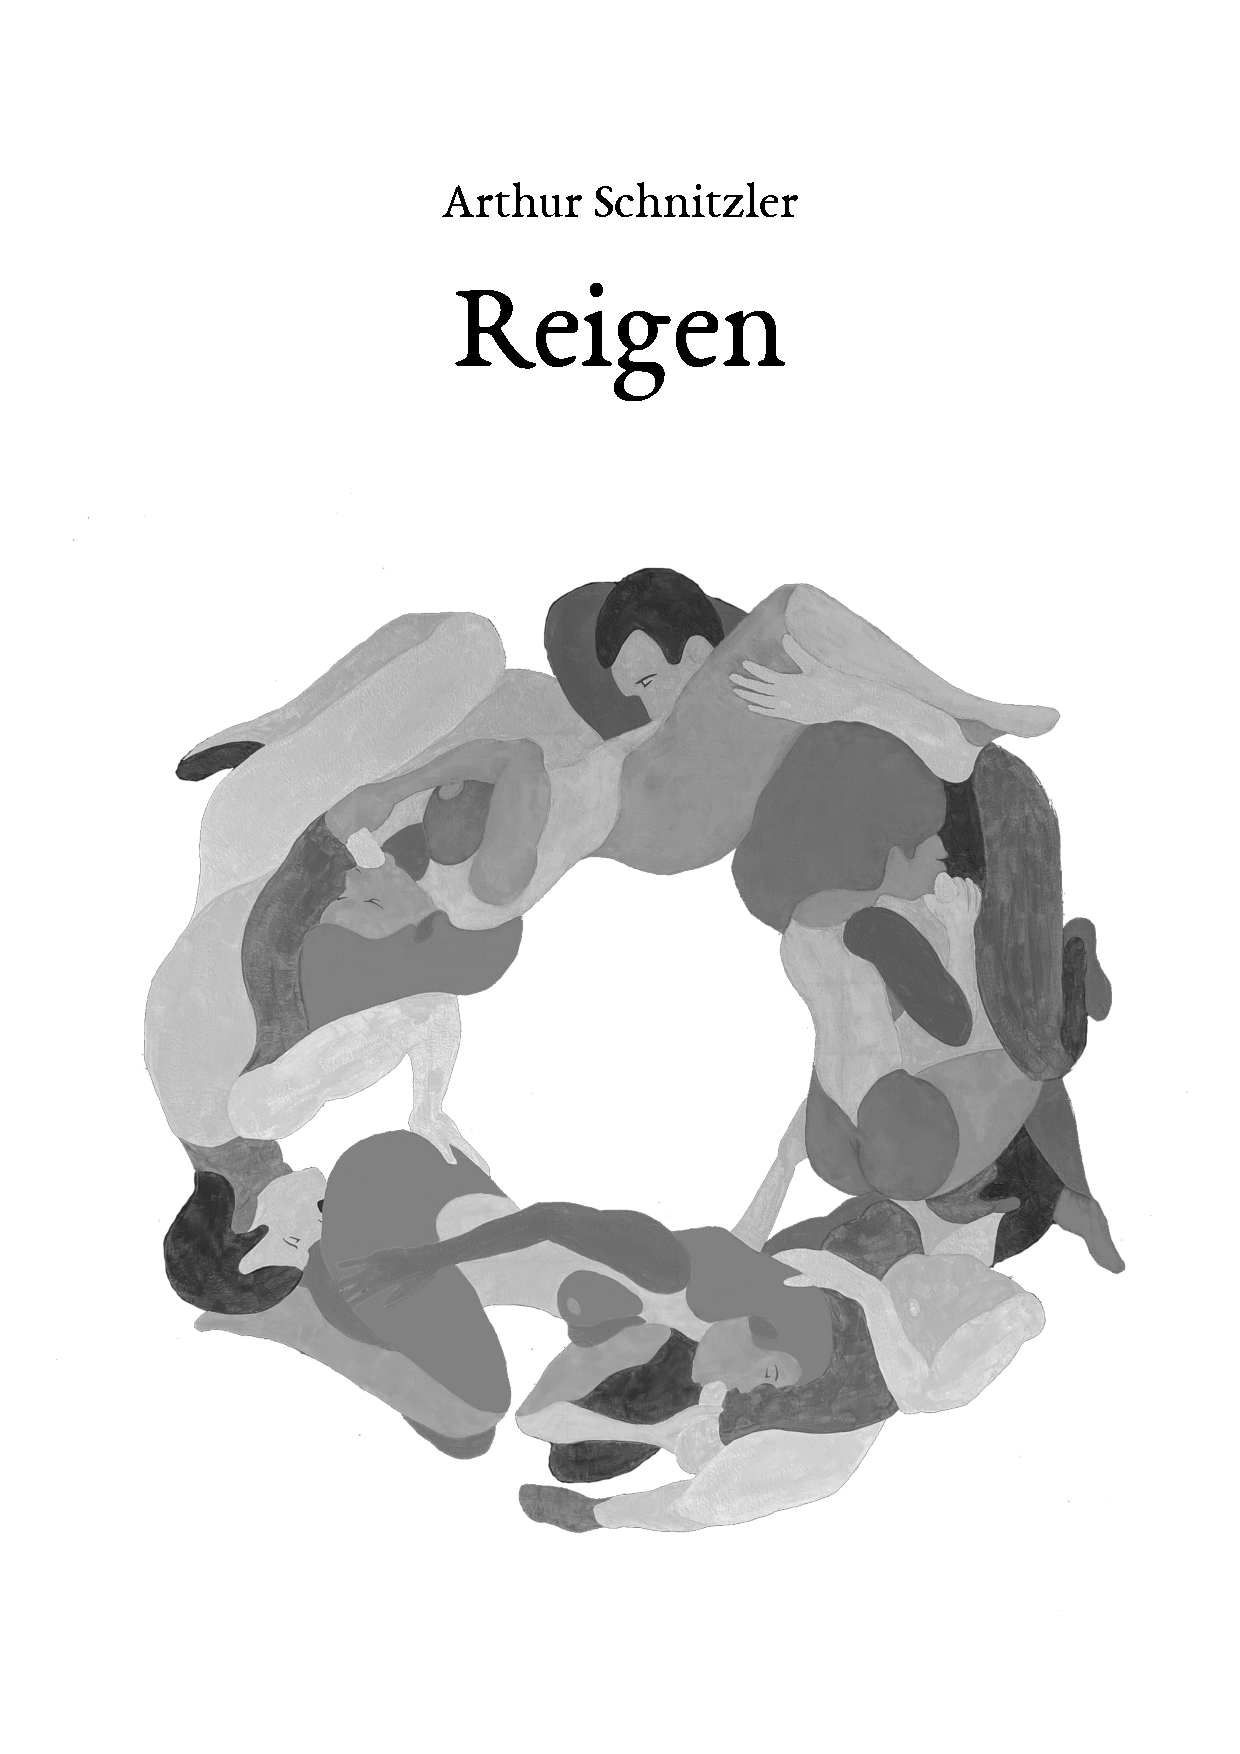
\includepdf{cover/cover}
\cleardoubleoddemptypage

\pagenumbering{roman}
\maketitle

\pdfbookmark[chapter]{\contentsname}{toc}
\tableofcontents
\cleardoubleoddpage

\pagestyle{headings}
\pagenumbering{arabic}
\doublespacing

\act{Erster Akt}
\scene{Die Nutte und die Soldatin.}
\characterlist{\thedirne, \thesoldat}
\setting{Spät abends. Am Straßenstrich.}
\begin{play}
	\soldat
	\direction{kommt pfeifend, will nach Hause.}

	\dirne
	Komm, mein schöner Engel.

	\soldat
	\direction{wendet sich um und geht wieder weiter.}

	\dirne
	Willst du nicht mit mir kommen?

	\soldat
	Ah, ich bin der schöne Engel?

	\dirne
	Freilich, wer denn? Geh, komm zu mir. Ich wohn gleich in der Näh.

	\soldat
	Ich hab keine Zeit. Ich muß in die Kasern!

	\dirne
	In die Kasern kommst immer noch zurecht. Bei mir is besser.

	\soldat
	\direction{ihr nahe.} Das ist schon möglich.

	\dirne
	Pst. Jeden Moment kann ein Wachmann kommen.

	\soldat
	Lächerlich! Wachmann! Ich hab auch mein Seiteng wehr!

	\dirne
	Geh, komm mit.

	\soldat
	Laß mich in Ruh, Geld hab ich eh keins.

	\dirne
	Ich brauch kein Geld.

	\soldat
	\direction{bleibt stehen. Sie sind bei einer Laterne.} Du brauchst kein Geld? Wer bist denn du nachher?

	\dirne
	Zahlen tun mir die Zivilisten. So einer wie du kanns immer umsonst bei mir haben.

	\soldat
	Du bist am End die, von der mir der Huber erzählt hat.

	\dirne
	Ich kenn kein Huber nicht.

	\soldat
	Du wirst schon die sein. Weißt --- in dem Kaffeehaus in der Schiffgassen --- von dort ist er mit dir z Haus gangen.

	\dirne
	Von dem Kaffeehaus bin ich schon mit gar vielen z Haus gangen \ldots{} oh! oh! ---

	\soldat
	Also gehn wir, gehn wir.

	\dirne
	Was, jetzt hasts eilig?

	\soldat
	Na, worauf solln wir noch warten? Und um zehn muß ich in der Kasern sein.

	\dirne
	Wie lang dienst denn schon?

	\soldat
	Was geht denn das dich an? Wohnst weit?

	\dirne
	Zehn Minuten zum gehn.

	\soldat
	Das ist mir zu weit. Gib mir ein Pussel.

	\dirne
	\direction{küßt ihn.} Das ist mir eh das liebste, wenn ich einen gern hab!

	\soldat
	Mir nicht. Nein, ich geh nicht mit dir, es ist mir zu weit.

	\dirne
	Weißt was, komm morgen am Nachmittag.

	\soldat
	Gut is. Gib mir deine Adresse.

	\dirne
	Aber du kommst am End nicht.

	\soldat
	Wenn ich dirs sag!

	\dirne
	Du, weißt was --- wenns dir zu weit ist heut abend zu mir --- da \ldots{} da \ldots{} \direction{weist auf die Donau.}

	\soldat
	Was ist das?

	\dirne
	Da ist auch schön ruhig \ldots{} jetzt kommt kein Mensch.

	\soldat
	Ah, das ist nicht das Rechte.

	\dirne
	Bei mir is immer das Rechte. Geh, bleib jetzt bei mir. Wer weiß, ob wir morgen nochs Leben haben.

	\soldat
	So komm --- aber g'schwind!

	\dirne
	Gib Obacht, da ist so dunkel. Wennst ausrutschst, liegst in der Donau.

	\soldat
	Wär eh das beste.

	\dirne
	Pst, so wart nur ein bissel. Gleich kommen wir zu einer Bank.

	\soldat
	Kennst dich da gut aus.

	\dirne
	So einen wie dich möcht ich zum Geliebten.

	\soldat
	Ich tät dir zu viel eifern.

	\dirne
	Das möcht ich dir schon abgewöhnen.

	\soldat
	Ha ---

	\dirne
	Nicht so laut. Manchmal is doch, daß sich ein Wachter her verirrt. Sollt man glauben, daß wir da mitten in der Wienerstadt sind?

	\soldat
	Daher komm, daher.

	\dirne
	Aber was fällt dir denn ein, wenn wir da ausrutschen, liegen wir im Wasser unten.

	\soldat
	\direction{hat sie gepackt.} Ah, du ---

	\dirne
	Halt dich nur fest an.

	\soldat
	Hab kein Angst \ldots{}

	\hiat

	\dirne
	Auf der Bank wärs schon besser gewesen.

	\soldat
	Da oder da \ldots{} Na, krall aufi.

	\dirne
	Was laufst denn so ---

	\soldat
	Ich muß in die Kasern, ich komm eh schon zu spät.

	\dirne
	Geh, du, wie heißt denn?

	\soldat
	Was interessiert dich denn das, wie ich heiß?

	\dirne
	Ich heiß Leocadia.

	\soldat
	Ha! --- So an Namen hab ich auch noch nie gehört.

	\dirne
	Du!

	\soldat
	Na, was willst denn?

	\dirne
	Geh, ein Sechserl fürn Hausmeister gib mir wenigstens! ---

	\soldat
	Ha! \ldots{} Glaubst, ich bin deine Wurzen. Servus! Leocadia \ldots{}

	\dirne
	Strizzi! Fallott! ---

	\direction{Er ist verschwunden.}

\end{play}

\scene{Die Soldatin und der Praktikant.}
\characterlist{\thesoldat, \thepraktikant}
\setting{Dorfdisko im Speckgürtel Berlins.}
\begin{play}


	\praktikant
	Jetzt sagen S' mir aber, warum S' durchaus schon haben fortgehen müssen.

	\soldat
	\direction{lacht verlegen, dumm.}

	\praktikant
	Es ist doch so schön gewesen. Ich tanz so gern.

	\soldat
	\direction{faßt sie um die Taille.}

	\praktikant
	\direction{läßts geschehen.} Jetzt tanzen wir ja nimmer. Warum halten S' mich so fest?

	\soldat
	Wie heißen S'? Kathi?

	\praktikant
	Ihnen ist immer eine Kathi im Kopf.

	\soldat
	Ich weiß, ich weiß schon \ldots{} Marie.

	\praktikant
	Sie, da ist aber dunkel. Ich krieg so eine Angst.

	\soldat
	Wenn ich bei Ihnen bin, brauchen S' Ihnen nicht zu fürchten. Gott sei Dank, mir sein mir!

	\praktikant
	Aber wohin kommen wir denn da? Da ist ja kein Mensch mehr. Kommen S', gehn wir zurück! --- Und so dunkel!

	\soldat
	\direction{zieht an seiner Virginierzigarre, daß das rote Ende leuchtet.} s' wird schon lichter! Haha! Oh, du Schatzerl!

	\praktikant
	Ah, was machen S' denn? Wenn ich das gewußt hätt!

	\soldat
	Also der Teufel soll mich holen, wenn eine heut beim Swoboda mollerter gewesen ist als Sie, Fräul'n Marie.

	\praktikant
	Haben S' denn bei allen so probiert?

	\soldat
	Was man so merkt, beim Tanzen. Da merkt man gar viel! Ha!

	\praktikant
	Aber mit der Blonden mit dem schiefen Gesicht haben S' doch mehr tanzt als mit mir.

	\soldat
	Das ist eine alte Bekannte von einem meinigen Freund.

	\praktikant
	Von dem Korporal mit dem aufdrehten Schnurrbart?

	\soldat
	Ah nein, das ist der Zivilist gewesen, wissen S', der im Anfang am Tisch mit mir g'sessen ist, der so heisrig redt.

	\praktikant
	Ah, ich weiß schon. Das ist ein kecker Mensch.

	\soldat
	Hat er Ihnen was tan? Dem möcht ichs zeigen! Was hat er Ihnen tan?

	\praktikant
	Oh, nichts --- ich hab nur gesehn, wie er mit die andern ist.

	\soldat
	Sagen S', Fräulein Marie \ldots{}

	\praktikant
	Sie werden mich verbrennen mit Ihrer Zigarrn.

	\soldat
	Pahdon! --- Fräul'n Marie. Sagen wir uns du.

	\praktikant
	Wir sein noch nicht so gute Bekannte.

	\soldat
	Es können sich gar viele nicht leiden und sagen doch du zueinander.

	\praktikant
	's nächstemal, wenn wir \ldots{} Aber, Herr Franz ---

	\soldat
	Sie haben sich meinen Namen g'merkt?

	\praktikant
	Aber, Herr Franz \ldots{}

	\soldat
	Sagen S' Franz, Fräulein Marie.

	\praktikant
	So sein S' nicht so keck --- aber pst, wenn wer kommen tät!

	\soldat
	Und wenn schon einer kommen tät, man sieht ja nicht zwei Schritt weit.

	\praktikant
	Aber um Gottes willen, wohin kommen wir denn da?

	\soldat
	Sehn S', da sind zwei grad wie mir.

	\praktikant
	Wo denn? Ich seh gar nichts.

	\soldat
	Da \ldots{} vor uns.

	\praktikant
	Warum sagen S' denn: zwei wie mir? ---

	\soldat
	Na, ich mein halt, die haben sich auch gern.

	\praktikant
	Aber geben S' doch acht, was ist denn da, jetzt wär ich beinah g'fallen.

	\soldat
	Ah, das ist das Gatter von der Wiesen.

	\praktikant
	Stoßen S' doch nicht so, ich fall ja um.

	\soldat
	Pst, nicht so laut.

	\praktikant
	Sie, jetzt schrei ich aber wirklich. --- Aber was machen S' denn \ldots{} aber ---

	\soldat
	Da ist jetzt weit und breit keine Seel.

	\praktikant
	So gehn wir zurück, wo Leut sein.

	\soldat
	Wir brauchen keine Leut, was, Marie, wir brauchen \ldots{} dazu \ldots{} haha.

	\praktikant
	Aber, Herr Franz, bitt Sie, um Gottes willen, schaun S', wenn ich das \ldots{} gewußt \ldots{} oh \ldots{} oh \ldots{} komm!

	\hiat

	\soldat
	\direction{selig.} Herrgott noch einmal \ldots{} ah \ldots{}

	\praktikant
	\ldots{} Ich kann dein G'sicht gar nicht sehn.

	\soldat
	A was --- G'sicht \ldots{}

	\hiat

	\soldat
	Ja, Sie, Fräul'n Marie, da im Gras können S' nicht liegenbleiben.

	\praktikant
	Geh, Franz, hilf mir.

	\soldat
	Na, komm zugi.

	\praktikant
	O Gott, Franz.

	\soldat
	Naja, was ist denn mit dem Franz?

	\praktikant
	Du bist ein schlechter Mensch, Franz.

	\soldat
	Ja, ja. Geh, wart ein bissel.

	\praktikant
	Was laßt mich denn aus?

	\soldat
	Na, die Virginier werd ich mir doch anzünden dürfen.

	\praktikant
	Es ist so dunkel.

	\soldat
	Morgen früh ist schon wieder licht.

	\praktikant
	Sag wenigstens, hast mich gern?

	\soldat
	Na, das mußt doch g'spürt haben, Fräul'n Marie, ha!

	\praktikant
	Wohin gehn wir denn?

	\soldat
	Na, zurück.

	\praktikant
	Geh, bitt dich, nicht so schnell!

	\soldat
	Na, was ist denn? Ich geh nicht gern in der finstern.

	\praktikant
	Sag, Franz, hast mich gern?

	\soldat
	Aber grad hab ichs gsagt, daß ich dich gern hab!

	\praktikant
	Geh, willst mir nicht ein Pussel geben?

	\soldat
	\direction{gnädig.} Da \ldots{} Hörst --- jetzt kann man schon wieder die Musik hören.

	\praktikant
	Du möchtst am End gar wieder tanzen gehn?

	\soldat
	Na freilich, was denn?

	\praktikant
	Ja, Franz, schau, ich muß zuhaus gehn.
	\begin{deletion}
		Sie werden eh schon schimpfen, mei Frau ist so eine \ldots{} die möcht am liebsten, man ging gar nicht fort.
	\end{deletion}

	\soldat
	Na ja, geh halt zuhaus.

	\praktikant
	Ich hab halt dacht, Herr Franz, Sie werden mich z'aus führen.

	\soldat
	Z'haus führen? Ah!

	\praktikant
	Gehn S', es ist so traurig, allein z'haus gehn.

	\soldat
	Wo wohnen S' denn?

	\praktikant
	Es ist gar nicht so weit --- in Teltow.

	\soldat
	So? Ja, da haben wir ja einen Weg \ldots{} aber jetzt ists mir zu früh \ldots{} jetzt wird noch draht, heut hab ich über Zeit \ldots{} vor zwölf brauch ich nicht in der Kasern zu sein. I geh noch tanzen.

	\praktikant
	Freilich, ich weiß schon, jetzt kommt die Blonde mit dem schiefen Gesicht dran!

	\soldat
	Ha! --- Der ihr G'sicht ist gar nicht so schief.

	\praktikant
	O Gott, sein die Männer schlecht. Was, Sie machens sicher mit einer jeden so.

	\soldat
	Das wär z'viel! ---

	\praktikant
	Franz, bitt schön, heut nimmer, --- heut bleiben S' mit mir, schaun S' ---

	\soldat
	Ja, ja, ist schon gut. Aber tanzen werd ich doch noch dürfen.

	\praktikant
	Ich tanz heut mit kein mehr!

	\soldat
	Da ist er ja schon \ldots{}

	\praktikant
	Wer denn?

	\soldat
	Der Swoboda! Wie schnell wir wieder da sein. Noch immer spielen s' das \ldots{} tadarada tadarada \ldots{} \direction{Singt mit.} \ldots{} Also, wanst auf mich warten willst, so führ ich dich z'haus \ldots{} wenn nicht \ldots{} Servus ---

	\praktikant
	Ja, ich werd warten.

	\direction{Sie treten in den Tanzsaal ein.}

	\soldat
	Wissen S', Fräul'n Marie, ein Glas Bier lassens Ihnen geben. \direction{Zu einer Blonden sich wendend, die eben mit einem Burschen vorbeitanzt, sehr hochdeutsch.} Mein Fräulein, darf ich bitten? ---

\end{play}

\scene{Der Praktikant und der Junge Herr}
\characterlist{\thepraktikant, \theherr}
\setting{Im Office eines Startups.}
\begin{play}
	\praktikant
	Bitt schön, junger Herr?

	\herr
	Ah ja, Marie, ah ja, ich hab geläutet, ja \ldots{} was hab ich nur \ldots{} ja richtig, die Rouletten lassen S' herunter, Marie \ldots{} Es ist kühler, wenn die Rouletten unten sind \ldots{} ja \ldots{}

	\direction{Das Stubenmädchen geht zum Fenster und läßt die Rouletten herunter.}

	\herr
	\direction{liest weiter.} Was machen S' denn, Marie? Ah ja. Jetzt sieht man aber gar nichts zum Lesen.

	\praktikant
	Der junge Herr ist halt immer so fleißig.

	\herr
	\direction{überhört das vornehm.} So, ist gut.

	\direction{Marie geht.}

	\herr
	\direction{versucht weiterzulesen; läßt bald das Buch fallen, klingelt wieder.}

	\praktikant
	\direction{erscheint.}

	\herr
	Sie, Marie \ldots{} ja, was ich habe sagen wollen \ldots{} ja \ldots{} ist vielleicht ein Bier zu Haus?

	\begin{deletion}
	\praktikant
	Ja, der wird eingesperrt sein.

	\herr
	Na, wer hat denn die Schlüssel?

	\praktikant
	Die Schlüssel hat die Lini.

	\herr
	Wer ist die Lini?

	\praktikant
	Die Köchin, Herr Alfred.

	\herr
	Na, so sagen S' es halt der Lini.

	\praktikant
	Ja, die Lini hat heut Ausgang.

	\herr
	So \ldots{}
	\end{deletion}

	\praktikant
	Soll ich dem jungen Herrn vielleicht aus dem Späti \ldots{}

	\herr
	Ah nein \ldots{} es ist so heiß genug. Ich brauch keine Bier. Wissen S', Marie, bringen Sie mir ein Glas Wasser. Pst, Marie --- aber laufen lassen, daß es recht kalt ist. ---

	\direction{\thepraktikant{} ab.}

	\herr
	\direction{richtet sich zur Hälfte auf, der \thepraktikant{} gibt ihm das Glas in die Hand, ihre Finger berühren sich.}

	\herr
	So, danke. --- Na, was ist denn? --- Geben Sie acht; stellen Sie das Glas wieder auf die Tasse \ldots{} \direction{Er legt sich hin und streckt sich aus.} Wie spät ists denn? ---

	\praktikant
	Fünf Uhr, junger Herr.

	\herr
	So, fünf Uhr. --- Ist gut. ---

	\praktikant
	\direction{geht; bei der Tür wendet sie sich um; der junge Herr hat ihr nachgeschaut; sie merkt es und lächelt.}

	\herr
	\direction{bleibt eine Weile liegen, dann steht er plötzlich auf. Er geht bis zur Tür, wieder zurück, legt sich auf den Diwan. Er versucht wieder zu lesen. Nach ein paar Minuten klingelt er wieder.}

	\praktikant
	\direction{erscheint mit einem Lächeln, das sie nicht zu verbergen sucht.}

	\herr
	Sie, Marie, was ich Sie hab fragen wollen. War heut vormittag nicht der Doktor Schüller da?

	\praktikant
	Nein, heut vormittag war niemand da.

	\herr
	So, das ist merkwürdig. Also der Doktor Schüller war nicht da? Kennen Sie überhaupt den Doktor Schüller?

	\praktikant
	Freilich. Das ist der große Herr mit dem schwarzen Vollbart.

	\herr
	Ja. War er vielleicht doch da?

	\praktikant
	Nein, es war niemand da, junger Herr.

	\herr
	\direction{entschlossen.} Kommen Sie her, Marie.

	\praktikant
	\direction{tritt etwas näher.} Bitt schön.

	\herr
	Näher \ldots{} so \ldots{} ah \ldots{} ich hab nur geglaubt \ldots{}

	\praktikant
	Was haben der junge Herr?

	\herr
	Geglaubt \ldots{} geglaubt hab ich --- Nur wegen Ihres T-Shirts \ldots{} Was ist das für eine \ldots{} Na, kommen S' nur näher. Ich beiß Sie ja nicht.

	\praktikant
	\direction{kommt zu ihm.} Was ist mit meinem T-Shirt? G'fallt sie dem jungen Herrn nicht?

	\herr
	\direction{faßt das T-Shirt an, wobei er das Stubenmädchen zu sich herabzieht.} Blau? Das ist ganz ein schönes Blau. \direction{Einfach.} Sie sind sehr nett angezogen, Marie.

	\praktikant
	Aber, junger Herr \ldots{}

	\herr
	Na, was ist denn? \ldots{} \direction{Er hat ihre Bluse geöffnet. Sachlich.} Sie haben eine schöne Haut, Marie.

	\praktikant
	Der junge Herr tut mir schmeicheln.

	\herr
	\direction{küßt sie auf die Brust.} Das kann doch nicht weh tun.

	\praktikant
	O nein.

	\herr
	Weil Sie so seufzen! Warum seufzen Sie denn?

	\praktikant
	Oh, Herr Alfred \ldots{}

	\begin{deletion}
	\herr
	Und was Sie für nette Pantoffeln haben \ldots{}
	\end{deletion}

	\praktikant
	\ldots{} Aber \ldots{} junger Herr 
	\begin{deletion}
		\ldots{} wenns draußen läut ---
	\end{deletion}
	\direction{kommt.}

	\herr
	Wer wird denn jetzt läuten?

	\praktikant
	Aber junger Herr \ldots{} schaun S' \ldots{} es ist so licht \ldots{}

	\herr
	Vor mir brauchen Sie sich nicht zu genieren. Sie brauchen sich überhaupt vor niemandem \ldots{} wenn man so hübsch ist. Ja, meiner Seel; Marie, Sie sind \ldots{} Wissen Sie, Ihre Haare riechen sogar angenehm.

	\begin{deletion}
	\praktikant
	Herr Alfred \ldots{}

	\herr
	Machen Sie keine solchen Geschichten, Marie \ldots{} ich hab Sie schon anders auch gesehn. Wie ich neulich in der Nacht nach Haus gekommen bin und mir Wasser geholt hab; da ist die Tür zu Ihrem Zimmer offen gewesen \ldots{} na \ldots{}
	\end{deletion}

	\praktikant
	\direction{verbirgt sein Gesicht.} O Gott, aber das hab ich gar nicht gewußt, daß der Herr Alfred so schlimm sein kann.

	\herr
	Da hab ich sehr viel gesehen \ldots{} das \ldots{} und das \ldots{} und das \ldots{} und ---

	\praktikant
	Aber, Herr Alfred!

	\herr
	Komm, komm \ldots{} daher \ldots{} so, ja so \ldots{}

	\praktikant
	Aber wenn jetzt wer läutet ---

	\herr
	Jetzt hören Sie schon einmal auf \ldots{} macht man höchstens nicht auf \ldots{}

	\hiat

	\direction{Es klingelt.}

	\herr
	Donnerwetter \ldots{} Und was der Kerl für einen Lärm macht. --- Am End hat der schon früher geläutet, und wir habens nicht gemerkt.

	\praktikant
	Oh, ich hab alleweil aufgepaßt.

	\herr
	Na, so schaun S' endlich nach --- durchs Guckerl.

	\praktikant
	Herr Alfred \ldots{} Sie sind aber \ldots{} nein \ldots{} so schlimm.

	\herr
	Bitt Sie, schaun S' jetzt nach \ldots{}

	\praktikant
	\direction{geht ab.}

	\herr
	\direction{öffnet rasch die Rouleaux.}

	\praktikant
	\direction{erscheint wieder.} Der ist jedenfalls schon wieder weggangen. Jetzt ist niemand mehr da. Vielleicht ist es der Doktor Schüller gewesen.

	\herr
	\direction{ist unangenehm berührt.} Es ist gut.

	\praktikant
	\direction{nähert sich ihm.}

	\herr
	\direction{entzieht sich ihr.} --- Sie, Marie, --- ich mach' jetzt Feierabend.

	\praktikant
	\direction{zärtlich.} Schon \ldots{} Herr Alfred.

	\herr
	\direction{streng.} Ich mach jetzt Feierabend.
	\begin{deletion}
		Wenn der Doktor Schüller kommen sollte ---

	\praktikant
	Der kommt heut nimmer.

	\herr
	\direction{noch strenger.} Wenn der Doktor Schüller kommen sollte, ich, ich \ldots{} ich bin --- im Kaffeehaus. --- \direction{Geht ins andere Zimmer.}
	\end{deletion}

	\direction{Der \thepraktikant{} nimmt eine Zigarrette, steckt sie ein und geht ab.}

\end{play}

\scene{Der junge Herr und die junge Frau.}
\characterlist{\theherr, \thefrau}
\setting{Im Office eines Startups. Die beiden sind Kollegen. Er bereitet sich auf ihr Eintreffen vor.}
\begin{play}

	\frau
	\direction{Sjjchließt die Tür hinter sich, bleibt einen Augenblick stehen, indem sie die linke Hand aufs Herz legt, als müsse sie eine gewaltige Erregung bemeistern.}

	\herr
	\direction{tritt auf sie zu, nimmt ihre linke Hand und drückt auf den weißen, schwarz tamburierten Handschuh einen Kuß. Er sagt leise.} Ich danke Ihnen.

	\frau
	Alfred --- Alfred!

	\herr
	Kommen Sie, gnädige Frau \ldots{} Kommen Sie, Frau Emma \ldots{}

	\frau
	Lassen Sie mich noch eine Weile --- bitte \ldots{} oh bitte sehr, Alfred! \direction{Sie steht noch immer an der Tür.}

	\herr
	\direction{steht vor ihr, hält ihre Hand.}

	\frau
	Wo bin ich denn eigentlich?

	\herr
	Bei mir.

	\frau
	Dieses Haus ist schrecklich, Alfred.

	\begin{deletion}
	\herr
	Warum denn? Es ist ein sehr vornehmes Haus.

	\frau
	Ich bin zwei Herren auf der Stiege begegnet.

	\herr
	Bekannte?

	\frau
	Ich weiß nicht. Es ist möglich.

	\herr
	Pardon, gnädige Frau --- aber Sie kennen doch Ihre Bekannten.

	\frau
	Ich habe ja gar nichts gesehen.

	\herr
	Aber wenn es selbst Ihre besten Freunde waren, --- sie können ja Sie nicht erkannt haben. Ich selbst \ldots{} wenn ich nicht wüßte, daß Sie es sind \ldots{} dieser Schleier ---

	\frau
	Es sind zwei.
	\end{deletion}

	\herr
	Wollen Sie nicht ein bißchen näher? \ldots{} Und Ihren Hut legen Sie doch wenigstens ab!

	\frau
	Was fällt Ihnen ein, Alfred? Ich habe Ihnen gesagt: Fünf Minuten \ldots{} Nein, länger nicht \ldots{} ich schwöre Ihnen ---

	\begin{deletion}
	\herr
	Also den Schleier ---

	\frau
	Es sind zwei.

	\herr
	Nun ja, beide Schleier --- ich werde Sie doch wenigstens sehen dürfen.

	\frau
	Haben Sie mich denn lieb, Alfred?

	\herr
	\direction{tief verletzt.} Emma --- Sie fragen mich \ldots{}

	\frau
	Es ist hier so heiß.

	\herr
	Aber Sie haben ja Ihre Pelzmantille an --- Sie werden sich wahrhaftig verkühlen.
	\end{deletion}

	\frau
	\direction{tritt endlich ins Zimmer, wirft sich auf den Fauteuil.} Ich bin totmüd.

	\herr
	Erlauben Sie. \direction{Er nimmt ihr die Jacke ab.}

	\frau
	\direction{läßt es geschehen.}

	\herr
	\direction{steht vor ihr, schüttelt den Kopf.}

	\frau
	Was haben Sie?

	\herr
	So schön waren Sie noch nie.

	\frau
	Wieso?

	\herr
	Allein \ldots{} allein mit Ihnen --- Emma --- \direction{Er läßt sich neben ihrem Fauteuil nieder, auf ein Knie, nimmt ihre beiden Hände und bedeckt sie mit Küssen.}

	\frau
	Und jetzt \ldots{} lassen Sie mich wieder gehen. Was Sie von mir verlangt haben, hab ich getan.

	\herr
	\direction{läßt seinen Kopf auf ihren Schoß sinken.}

	\frau
	Sie haben mir versprochen, brav zu sein.

	\herr
	Ja.

	\frau
	Man erstickt in diesem Zimmer.
	\begin{deletion}
	\herr
	\direction{steht auf.} Noch haben Sie Ihre Mantille an.

	\frau
	Legen Sie sie zu meinem Hut.

	\herr
	\direction{nimmt ihr die Mantille ab und legt sie gleichfalls auf den Diwan.}

	\frau
	Und jetzt --- adieu ---

	\herr
	Emma ---! Emma! ---

	\frau
	\end{deletion}
	Die fünf Minuten sind längst vorbei.

	\herr
	Noch nicht eine! ---

	\frau
	Alfred, sagen Sie mir einmal ganz genau, wie spät es ist.

	\herr
	Es ist Punkt viertel nach sechs.

	\frau
	Jetzt sollte ich längst bei meiner Schwester sein.

	\herr
	Ihre Schwester können Sie oft sehen \ldots{}

	\frau
	O Gott, Alfred, warum haben Sie mich dazu verleitet.

	\herr
	Weil ich Sie \ldots{} anbete, Emma.

	\frau
	Wie vielen haben Sie das schon gesagt?

	\herr
	Seit ich Sie gesehen, niemandem.

	\frau
	Was bin ich für eine leichtsinnige Person! Wer mir das vorausgesagt hätte \ldots{} noch vor acht Tagen \ldots{} noch gestern \ldots{}

	\herr
	Und vorgestern haben Sie mir ja schon versprochen \ldots{}

	\frau
	Sie haben mich so gequält. Aber ich habe es nicht tun wollen. Gott ist mein Zeuge --- ich habe es nicht tun wollen \ldots{} Gestern war ich fest entschlossen \ldots{}

	\begin{deletion}
	Wissen Sie, daß ich Ihnen gestern abend sogar einen langen Brief geschrieben habe?

	\herr
	Ich habe keinen bekommen.

	\frau
	Ich habe ihn wieder zerrissen. Oh, ich hätte Ihnen lieber diesen Brief schicken sollen.

	\herr
	Es ist doch besser so.
	\end{deletion}

	\frau
	O nein, es ist schändlich \ldots{} von mir. Ich begreife mich selber nicht. Adieu, Alfred, lassen Sie mich.

	\herr
	\direction{umfaßt sie und bedeckt ihr Gesicht mit heißen Küssen.}

	\frau
	So \ldots{} halten Sie Ihr Wort \ldots{}

	\herr
	Noch einen Kuß --- noch einen.

	\frau
	Den letzten. \direction{Er küßt sie; sie erwidert den Kuß; ihre Lippen bleiben lange aneinandergeschlossen.}

	\herr
	Soll ich Ihnen etwas sagen, Emma? Ich weiß jetzt erst, was Glück ist.

	\frau
	\direction{sinkt in einen Fauteuil zurück.}

	\herr
	\direction{setzt sich auf die Lehne, schlingt einen Arm leicht um ihren Nacken.} \ldots{} oder vielmehr, ich weiß jetzt erst, was Glück sein könnte.

	\frau
	\direction{seufzt tief auf.}

	\herr
	\direction{küßt sie wieder.}

	\frau
	Alfred, Alfred, was machen Sie aus mir!

	\herr
	Nicht wahr --- es ist hier gar nicht so ungemütlich \ldots{} Und wir sind ja hier so sicher! Es ist doch tausendmal schöner als diese Rendezvous im Freien \ldots{}

	\frau
	Oh, erinnern Sie mich nur nicht daran.

	\herr
	Ich werde auch daran immer mit tausend Freuden denken. Für mich ist jede Minute, die ich an Ihrer Seite verbringen durfte, eine süsse Erinnerung.

	\frau
	Erinnern Sie sich noch an den Industriellenball?

	\herr
	Ob ich mich daran erinnere \ldots{}? Da bin ich ja während des Soupers neben Ihnen gesessen, ganz nahe neben Ihnen. Ihr Mann hat Champagner \ldots{}

	\frau
	\direction{sieht ihn klagend an.}

	\marginnote{\enquote{Für dich auch eine Nase, mein Hase?}}
	\herr
	Ich wollte nur vom Champagner reden. Sagen Sie, Emma, wollen Sie nicht ein Glas Cognac trinken?

	\frau
	Einen Tropfen
	\begin{deletion}
		, aber geben Sie mir vorher ein Glas Wasser.
	\end{deletion}

	\herr
	Ja \ldots{} Wo ist denn nur --- ach ja \ldots{} \direction{Er schlägt die Portiere zurück und geht ins Schlafzimmer.}

	\begin{deletion}
	\frau
	\direction{sieht ihm nach.}

	\herr
	\direction{kommt zurück mit einer Karaffe Wasser und zwei Trinkgläsern.}

	\frau
	Wo waren Sie denn?

	\herr
	Im \ldots{} Nebenzimmer. \direction{Schenkt ein Glas Wasser ein.}
	\end{deletion}

	\frau
	Jetzt werde ich Sie etwas fragen, Alfred --- und schwören Sie mir, daß Sie mir die Wahrheit sagen werden.

	\herr
	Ich schwöre. ---

	\frau
	War in diesen Räumen schon jemals eine andere Frau?

	\herr
	Aber Emma --- dieses Haus steht schon zwanzig Jahre!

	\frau
	Sie wissen, was ich meine, Alfred \ldots{} Mit Ihnen! Bei Ihnen!

	\begin{deletion}
	\herr
	Mit mir --- hier --- Emma! --- Es ist nicht schön, daß Sie an so etwas denken können.

	\frau
	Also Sie haben \ldots{} wie soll ich \ldots{} Aber nein, ich will Sie lieber nicht fragen. Es ist besser, wenn ich nicht frage. Ich bin ja selbst schuld. Alles rächt sich.

	\herr
	Ja, was haben Sie denn? Was ist Ihnen denn? Was rächt sich?

	\frau
	Nein, nein, nein, ich darf nicht zum Bewußtsein kommen \ldots{} Sonst müßte ich vor Scham in die Erde sinken.
	\end{deletion}

	\herr
	\direction{mit der Karaffe Wasser in der Hand, schüttelt traurig den Kopf.} Emma, wenn Sie ahnen könnten, wie weh Sie mir tun.

	\frau
	\direction{schenkt sich ein Glas Cognac ein.}

	\herr
	Ich will Ihnen etwas sagen, Emma. Wenn Sie sich schämen, hier zu sein --- wenn ich Ihnen also gleichgültig bin --- wenn Sie nicht fühlen, daß Sie für mich alle Seligkeit der Welt bedeuten --- --- so gehn Sie lieber.

	\frau
	Ja, das werd ich auch tun.

	\begin{deletion}
	\herr
	\direction{sie bei der Hand fassend.} Wenn Sie aber ahnen, daß ich ohne Sie nicht leben kann, daß ein Kuß auf Ihre Hand für mich mehr bedeutet als alle Zärtlichkeiten, die alle Frauen auf der ganzen Welt \ldots{} Emma, ich bin nicht wie die anderen jungen Leute, die den Hof machen können --- ich bin vielleicht zu naiv \ldots{} ich \ldots{}

	\frau
	Wenn Sie aber doch sind wie die anderen jungen Leute?

	\herr
	Dann wären Sie heute nicht da --- denn Sie sind nicht wie die anderen Frauen.

	\frau
	Woher wissen Sie das?
	\end{deletion}

	\herr
	\begin{deletion}
		\direction{hat sie zum Diwan gezogen, sich nahe neben sie gesetzt.}
	\end{deletion}
	Ich habe viel über Sie nachgedacht. Ich weiß, Sie sind unglücklich.

	\frau
	\direction{erfreut.}

	\herr
	Das Leben ist so leer, so nichtig --- und dann --- so kurz --- so entsetzlich kurz! Es gibt nur ein Glück \ldots{} einen Menschen finden, von dem man geliebt wird ---

	\frau
	\direction{hat eine kandierte Birne vom Tisch genommen, nimmt sie in den Mund.}

	\herr
	Mir die Hälfte! \direction{Sie reicht sie ihm mit den Lippen.}

	\frau
	\direction{faßt die Hände des jungen Herrn, die sich zu verirren drohen.} Was tun Sie denn, Alfred \ldots{} Ist das Ihr Versprechen?

	\herr
	\direction{die Birne verschluckend, dann kühner.} Das Leben ist so kurz.

	\frau
	\direction{schwach.} Aber das ist ja kein Grund ---

	\herr
	\direction{mechanisch.} O ja.

	\frau
	\direction{schwächer.} Schauen Sie, Alfred, und Sie haben doch versprochen, brav \ldots{}
	\begin{deletion}
	Und es ist so hell \ldots{}

	\herr
	Komm, komm, du einzige, einzige \ldots{} \direction{Er hebt sie vom Diwan empor.}

	\frau
	Was machen Sie denn?

	\herr
	Da drin ist es gar nicht hell.

	\frau
	Ist denn da noch ein Zimmer?

	\herr
	\direction{zieht sie mit.} Ein schönes \ldots{} und ganz dunkel.

	\frau
	Bleiben wir doch lieber hier.

	\herr
	\direction{bereits mit ihr hinter der Portiere, im Schlafzimmer, nestelt ihr die Taille auf.}

	\frau
	\end{deletion}
	Sie sind so \ldots{} o Gott, was machen Sie aus mir! --- Alfred!

	\herr
	Ich bete dich an, Emma!

	\frau
	So wart doch, wart doch wenigstens \ldots{} \direction{Schwach.} Geh \ldots{} ich ruf dich dann.

	\herr
	Laß mir dich --- laß dir mich ---\direction{ Er verspricht sich.} \ldots{} laß \ldots{} mich --- dir --- helfen.

	\frau
	Du zerreißt mir ja alles.

	\herr
	Du hast kein Höschen an?

	\frau
	Ich trag nie ein Höschen. Die Odilon trägt auch keines. Aber die Schuh kannst du mir aufknöpfeln.

	\herr
	\direction{knöpfelt die Schuhe auf, küßt ihre Füße.}

	\frau
	\direction{ist ins Bett geschlüpft.} Oh, mir ist kalt.

	\herr
	Gleich wirds warm werden.

	\frau
	\direction{leise lachend.} Glaubst du?

	\herr
	\direction{unangenehm berührt, für sich.} Das hätte sie nicht sagen sollen. \direction{Entkleidet sich im Dunkel.}

	\frau
	\direction{zärtlich.} Komm, komm, komm!

	\herr
	\direction{dadurch wieder in besserer Stimmung.} Gleich --- ---

	\frau
	Es riecht hier so nach Veilchen.

	\herr
	Das bist du selbst \ldots{} Ja --- \direction{Zu ihr.} --- du selbst.

	\frau
	Alfred \ldots{} Alfred!!!!

	\herr
	Emma \ldots{}

	\marginnote{Er bekommt keinen hoch.}
	\hiat

	\herr
	Ich habe dich offenbar zu lieb \ldots{} ja \ldots{} ich bin wie von Sinnen.

	\frau
	\ldots{}

	\herr
	Die ganzen Tage über bin ich schon wie verrückt. Ich hab es geahnt.

	\frau
	Mach dir nichts draus.

	\herr
	O gewiß nicht. Es ist ja geradezu selbstverständlich, wenn man \ldots{}

	\frau
	Nicht \ldots{} nicht \ldots{} Du bist nervös. Beruhige dich nur \ldots{}

	\herr
	Kennst du Erich Fromm?

	\frau
	Fromm?

	\herr
	\enquote{Die Kunst des Liebens}

	\frau
	Nein, warum fragst du mich?

	\herr
	Da kommt eine Geschichte drin vor, die sehr bezeichnend ist.

	\frau
	Was ist das für eine Geschichte?

	\begin{deletion}
	\herr
	Das ist eine ganze Gesellschaft von Kavallerieoffizieren zusammen ---

	\frau
	So.
	\end{deletion}

	\herr
	Die erzählen von ihren Liebesabenteuern. Und jeder berichtet, daß ihm bei der Frau, die er am meisten, weißt du, am leidenschaftlichsten geliebt hat \ldots{} daß ihn die, daß er die --- also kurz und gut, daß es jedem bei dieser Frau so gegangen ist wie jetzt mir.

	\frau
	Ja.

	\herr
	Das ist sehr charakteristisch.

	\frau
	Ja.
	\begin{deletion}

	\herr
	Es ist noch nicht aus. Ein einziger behauptet \ldots{} es sei ihm in seinem ganzen Leben noch nicht passiert, aber, setzt Stendhal hinzu --- das war ein berüchtigter Bramarbas.

	\frau
	\end{deletion}
	So. ---

	\herr
	Und doch verstimmt es einen, das ist das Dumme, so gleichgültig es eigentlich ist.

	\frau
	Freilich. Überhaupt weißt du \ldots{} du hast mir ja versprochen, brav zu sein.

	\herr
	Geh, nicht lachen, das bessert die Sache nicht.

	\frau
	Aber nein, ich lache ja nicht. Die Geschichte ist wirklich interessant. Ich habe immer gedacht, daß nur bei älteren \ldots{} oder bei sehr \ldots{} weißt du, bei Leuten, die viel gelebt haben \ldots{}

	\herr
	Was fällt dir ein. Das hat damit gar nichts zu tun. Ich habe übrigens die hübscheste Geschichte ganz vergessen. Da ist einer von, der erzählt sogar, daß er drei Nächte oder gar sechs \ldots{} ich weiß nicht mehr, mit einer Frau zusammen war, die er durch Wochen hindurch verlangt hat --- désirée --- verstehst du --- und die haben alle diese Nächte hin durch nichts getan als vor Glück geweint \ldots{} beide \ldots{}

	\frau
	Beide?

	\herr
	Ja. Wundert dich das? Ich find das so begreiflich --- gerade wenn man sich liebt.

	\frau
	Aber es gibt gewiß viele, die nicht weinen.

	\herr
	\direction{nervös.} Gewiß \ldots{} das ist ja auch ein exceptioneller Fall.

	\frau
	Ah --- ich dachte, alle weinen bei dieser Gelegenheit.

	\herr
	Siehst du, jetzt machst du dich doch lustig.

	\frau
	Aber was fällt dir ein! Sei doch nicht kindisch, Alfred!

	\herr
	Es macht nun einmal nervös \ldots{} Dabei habe ich die Empfindung, daß du ununterbrochen daran denkst. Das geniert mich erst recht.

	\frau
	Ich denke absolut nicht daran.

	\herr
	O ja. Wenn ich nur überzeugt wäre, daß du mich liebst.

	\frau
	Verlangst du noch mehr Beweise?

	\herr
	Siehst du \ldots{} immer machst du dich lustig.

	\frau
	Wieso denn? Komm, gib mir dein süsses Kopferl.

	\herr
	Ach, das tut wohl.

	\frau
	Willst du mich?

	\herr
	Oh, ich bin ja so glücklich.

	\frau
	Aber du brauchst nicht auch noch zu weinen.

	\herr
	\direction{sich von ihr entfernend, höchst irritiert.} Wieder, wieder. Ich hab dich ja so gebeten \ldots{}

	\frau
	Wenn ich dir sage, daß du nicht weinen sollst \ldots{}

	\herr
	Du hast gesagt: auch noch zu weinen.

	\frau
	Du bist nervös, mein Schatz.

	\herr
	Das weiß ich.

	\frau
	Aber du sollst es nicht sein. Es ist mir sogar ganz recht. Lass' uns Freunde bleiben.
	\begin{deletion}

	\herr
	Schon wieder fangst du an.

	\frau
	Erinnerst du dich denn nicht! Das war eines unserer ersten Gespräche. Gute Kameraden haben wir sein wollen; nichts weiter. Oh, das war schön \ldots{} das war bei meiner Schwester, im Jänner auf dem großen Ball, während der Quadrille \ldots{} Um Gottes willen, ich sollte ja längst fort sein \ldots{} meine Schwester erwartet mich ja --- was werd ich ihr denn sagen \ldots{}
	\end{deletion}
	Adieu, Alfred ---

	\herr
	Emma ---! So willst du mich verlassen!

	\frau
	Ja --- so! ---

	\herr
	Noch fünf Minuten \ldots{}

	\marginnote{Sie bläst ihm halt noch einen, damit es nicht so awkward ist.}
	\frau
	Gut. Noch fünf Minuten. Aber du mußt mir versprechen dich nicht zu rühren? \ldots{} Ja? \ldots{} Ich will dir noch einen Kuß zum Abschied geben \ldots{} Pst \ldots{} ruhig \ldots{} nicht rühren, hab ich gesagt, sonst steh ich gleich auf, du mein süsser \ldots{} süsser \ldots{}

	\herr
	Emma \ldots{} meine ange \ldots{}

	\hiat

	\frau
	Mein Alfred ---

	\begin{deletion}
	\herr
	Ah, bei dir ist der Himmel.

	\frau
	Aber jetzt muß ich wirklich fort.

	\herr
	Ach, laß deine Schwester warten.

	\frau
	Nach Haus muß ich. Für meine Schwester ists längst zu spät. Wieviel Uhr ist es denn eigentlich?

	\herr
	Ja, wie soll ich das eruieren?

	\frau
	Du mußt eben auf die Uhr sehen.

	\herr
	Meine Uhr ist in meinem Gilet.

	\frau
	So hol sie.

	\herr
	\direction{steht mit einem mächtigen Ruck auf.} Acht.

	\frau
	\direction{erhebt sich rasch.} Um Gottes willen \ldots{} Rasch, Alfred, gib mir meine Strümpfe. Was soll ich denn nur sagen? Zu Hause wird man sicher schon auf mich warten \ldots{} acht Uhr \ldots{}
	\end{deletion}

	\herr
	Wann seh ich dich denn wieder?

	\frau
	Nie.

	\herr
	Emma! Willst du  mich denn nicht?

	\begin{deletion}
	\frau
	Eben darum. Gib mir meine Schuhe.

	\herr
	Niemals wieder? Hier sind die Schuhe.

	\frau
	In meinem Sack ist ein Schuhknöpfler. Ich bitt dich, rasch \ldots{}

	\herr
	Hier ist der Knöpfler.
	\end{deletion}

	\frau
	Alfred, das kann uns beide den Hals kosten.

	\herr
	\direction{höchst unangenehm berührt.} Wieso?

	\frau
	Ja, was soll ich denn sagen, wenn er mich fragt: Woher kommst du?

	\herr
	Von der Schwester.

	\frau
	Ja, wenn ich lügen könnte.

	\herr
	Na, du mußt es eben tun.

	\frau
	Alles für so einen Menschen. Ach, komm her \ldots{} laß dich noch einmal küssen. \direction{Sie umarmt ihn.} ---
	\begin{deletion}
	Und jetzt --- --- laß mich allein, geh ins andere Zimmer. Ich kann mich nicht anziehen, wenn du dabei bist.

	\herr
	\direction{geht in den Salon, wo er sich ankleidet. Er ißt etwas von der Bäckerei, trinkt ein Glas Cognac.}

	\frau
	\direction{ruft nach einer Weile.} Alfred!

	\herr
	Mein Schatz.

	\end{deletion}
	\frau
	Es ist doch besser, daß wir nicht geweint haben.

	\herr
	\direction{nicht ohne Stolz lächelnd.} Wie kann man so frivol reden ---

	\frau
	Wie wird das jetzt nur sein --- wenn wir uns zufällig wieder einmal in Gesellschaft begegnen?

	\herr
	Zufällig --- einmal \ldots{} Du bist ja morgen sicher auch auf Arbeit?

	\frau
	Ja. Du auch?

	\herr
	Freilich. Darf ich dich um den Kotillon bitten?

	\frau
	Oh, ich werde nicht hinkommen. Was glaubst du denn? --- Ich würde ja \ldots{} \direction{Sie tritt völlig angekleidet in den Salon, nimmt eine Schokoladenbäckerei.} \ldots{} in die Erde sinken.

	\herr
	Also morgen bei Lobheimer, das ist schön.

	\frau
	Nein, nein \ldots{} ich sage ab; bestimmt ---

	\herr
	Also übermorgen \ldots{} hier.

	\frau
	Was fällt dir ein?

	\herr
	Um sechs \ldots{}

	\frau
	Hier an der Ecke stehen Wagen, nicht wahr? ---

	\herr
	Ja, so viel du willst. Also übermorgen hier um sechs. So sag doch ja, mein geliebter Schatz.

	\frau
	\ldots{} Das besprechen wir morgen beim Kotillon.

	\herr
	\direction{umarmt sie.} Mein Engel.

	\frau
	Nicht wieder meine Frisur ruinieren.

	\herr
	Also morgen bei Lobheimers und übermorgen in meinen Armen.

	\frau
	Leb wohl \ldots{}

	\herr
	\direction{plötzlich wieder besorgt.} Und was wirst du --- ihm heut sagen? ---

	\frau
	Frag nicht \ldots{} frag nicht \ldots{} es ist zu schrecklich. --- Warum hab ich dich so lieb! --- Adieu. --- Wenn ich wieder Menschen auf der Stiege begegne, trifft mich der Schlag. --- Pah! ---

	\herr
	\direction{küßt ihr noch einmal die Hand.}

	\frau
	\direction{geht.}

	\herr
	\direction{bleibt allein zurück. Dann setzt er sich auf den Diwan. Er lächelt vor sich hin und sagt zu sich selbst.} Also jetzt hab ich ein Verhältnis mit einer anständigen Frau.

\end{play}

\scene{Die junge Frau und der Gatte.}
\characterlist{\thefrau, \thegatte}
\begin{deletion}
\setting{Ein behagliches Schlafgemach. Es ist halb elf Uhr nachts. Die Frau liegt zu Bette und liest. Der Gatte tritt eben, im Schlafrock, ins Zimmer.}
\end{deletion}
\setting{Die \thefrau liegt im Bett und liest.}

\begin{play}

	\frau
	\direction{ohne aufzuschauen.} Du arbeitest nicht mehr?

	\gatte
	Nein. Ich bin zu müde.
	\begin{deletion}
	Und außerdem \ldots{}
	\end{deletion}

	\frau
	Nun? ---

	\gatte
	Ich hab mich an meinem Schreibtisch plötzlich so einsam gefühlt. Ich habe Sehnsucht nach dir bekommen.

	\frau
	\direction{schaut auf.} Wirklich?

	\gatte
	\direction{setzt sich zu ihr aufs Bett.} Lies heute nicht mehr.
	\begin{deletion}
	Du wirst dir die Augen verderben.
	\end{deletion}

	\frau
	\direction{schlägt das Buch zu.} Was hast du denn?

	\gatte
	Nichts, mein Schatz. Verliebt bin ich in dich! Das weißt du doch!

	\frau
	Man könnte es manchmal fast vergessen.

	\gatte
	Man muß es sogar manchmal vergessen.

	\frau
	Warum?

	\gatte
	Weil die Ehe sonst etwas Unvollkommenes wäre. Sie würde \ldots{}
	\begin{deletion}
		wie soll ich nur sagen \ldots{}
	\end{deletion}
	sie würde ihre Heiligkeit verlieren.

	\frau
	Oh \ldots{}

	\gatte
	Glaube mir --- es ist so \ldots{} Hätten wir in den fünf Jahren, die wir jetzt miteinander verheiratet sind, nicht manchmal vergessen, daß wir ineinander verliebt sind --- wir wären es wohl gar nicht mehr.

	\frau
	Das ist mir zu hoch.

	\gatte
	Die Sache ist
	\begin{deletion}
		einfach
	\end{deletion}
	die: wir haben vielleicht schon zehn oder zwölf miteinander geschlafen, oder?\ldots{}
	\begin{deletion}
		Kommt es dir nicht auch so vor?
	\end{deletion}

	\frau
	Ich hab nicht gezählt! ---

	\gatte
	Hätten wir gleich das erste Mal bis zum Ende ausgekostet, hätte ich mich von Anfang an meiner Leidenschaft für dich willenlos hingegeben, dann wäre ese uns wie den Millionen von anderen Liebespaaren ergangen. Wir wären fertig miteinander.

	\frau
	Ah \ldots{} so meinst du das?

	\gatte
	Glaube mir --- Emma --- in den ersten Tagen unserer Ehe hatte ich Angst, daß es so kommen würde.

	\frau
	Ich auch.

	\gatte
	Siehst du? Hab ich nicht recht gehabt? Darum ist es gut, immer wieder für einige Zeit nur in guter Freundschaft miteinander hinzuleben.

	\frau
	Ach so.

	\gatte
	Und so kommt es, daß wir immer wieder neue Flitterwochen miteinander durchleben können, da ich es nie drauf ankommen lasse, die Flitterwochen \ldots{}

	\frau
	Zu Monaten auszudehnen.

	\gatte
	Richtig.

	\frau
	Und jetzt \ldots{} scheint also wieder eine Freundschaftsperiode abgelaufen zu sein ---?

	\gatte
	\direction{sie zärtlich an sich drückend.} Es dürfte so sein.

	\frau
	Wenn es aber \ldots{} bei mir anders wäre.

	\gatte
	Es ist bei dir nicht anders. Du bist ja das klügste und entzückendste Wesen, das es gibt. Ich bin sehr glücklich, daß ich dich gefunden habe.

	\frau
	Das ist aber nett, wie du den Hof machen kannst --- von Zeit zu Zeit.

	\gatte
	\direction{hat sich auch zu Bett begeben.} Für einen Mann, der sich ein bißchen in der Welt umgesehen hat \direction{er bedeutet ihr, sie solle sich an ihn lehnen}, bedeutet die Ehe eigentlich etwas viel Geheimnisvolleres als für euch junge Mädchen aus guter Familie.
	\begin{deletion}
		Ihr tretet uns rein und \ldots{} wenigstens bis zu einem gewissen Grad unwissend entgegen, und darum habt ihr eigentlich einen viel klareren Blick für das Wesen der Liebe als wir.
	\end{deletion}

	\frau
	\direction{lachend.} Oh!

	\gatte
	Gewiß. Denn wir sind ganz verwirrt und unsicher geworden durch die vielfachen Erlebnisse, die wir notgedrungen vor der Ehe durchzumachen haben.
	\begin{deletion}
		Ihr hört ja viel und wißt zu viel und lest ja wohl eigentlich auch zu viel, aber einen rechten Begriff von dem, was wir Männer in der Tat erleben, habt ihr ja doch nicht.
	\end{deletion}
	Uns wird das, was man so gemeinhin die Liebe nennt, recht gründlich widerwärtig gemacht; denn was sind das schließlich für Geschöpfe, auf die wir angewiesen sind!

	\frau
	Ja, was sind das für Geschöpfe?

	\gatte
	\direction{küßt sie auf die Stirn.} Sei froh, mein Kind, daß du nie einen Einblick in diese Verhältnisse erhalten hast. Es sind übrigens meist recht bedauernswerte Wesen.
	\begin{deletion}
	--- werfen wir keinen Stein auf sie.

	\frau
	Bitt dich --- dieses Mitleid. --- Das kommt mir da gar nicht recht angebracht vor.

	\gatte
	\direction{mit schöner Milde.} Sie verdienen es. Ihr, die ihr junge Mädchen aus guter Familie wart, die ruhig unter Obhut euerer Eltern auf den Ehrenmann warten konntet, der euch zur Ehe begehrt; ---
	\end{deletion}
	Ihr Frauen kennt ja das Elend nicht, das die meisten von diesen armen Geschöpfen der Sünde in die Arme treibt.

	\begin{deletion}
	\frau
	So verkaufen sich denn alle?

	\gatte
	Das möchte ich nicht sagen. Ich mein ja auch nicht nur das materielle Elend. Aber es gibt auch --- ich möchte sagen --- ein sittliches Elend; eine mangelhafte Auffassung für das, was erlaubt, und insbesondere für das, was edel ist.
	\end{deletion}

	\frau
	Aber warum sind die zu bedauern? --- Denen gehts ja ganz gut?

	\gatte
	Du hast sonderbare Ansichten, mein Kind. Du darfst nicht vergessen, daß solche Wesen von Natur aus bestimmt sind, immer tiefer und tiefer zu fallen. Da gibt es kein Aufhalten.

	\frau
	\direction{sich an ihn schmiegend.} Offenbar fällt es sich ganz angenehm.

	\gatte
	\direction{peinlich berührt.} Wie kannst du so reden, Emma. Ich denke doch, daß es gerade für euch, anständige Frauen, nichts Widerwärtigeres geben kann als alle diejenigen, die es nicht sind.

	\frau
	Freilich, Karl, freilich. Ich habs ja auch nur so gesagt. Geh, erzähl
	\begin{deletion}
	weiter. Es ist so nett, wenn du so redst. Erzähl mir was.

	\gatte
	Was denn? ---

	\frau
	Nun ---
	\end{deletion}
	von diesen Geschöpfen.

	\gatte
	Was fällt dir denn ein?

	\frau
	Schau, ich hab dich schon früher
	\begin{deletion}
		, weißt du, ganz im Anfang hab ich dich immer
	\end{deletion}
	gebeten, du sollst mir aus deiner Jugend was erzählen.

	\gatte
	Warum interessiert dich denn das?

	\frau
	Bist du denn nicht mein Mann? Und ist das nicht geradezu eine Ungerechtigkeit, daß ich von deiner Vergangenheit eigentlich gar nichts weiß? ---

	\gatte
	Du wirst mich doch nicht für so geschmacklos halten, daß ich --- Genug, Emma \ldots{} das ist ja wie eine Entweihung.

	\frau
	\begin{deletion}
		Und doch hast du \ldots{}
	\end{deletion}
	Wer weiß wieviel andere Frauen du gerade so in den Armen gehalten wie jetzt mich.

	\gatte
	Sag doch nicht \emph{Frauen}. Frau bist du.

	\frau
	Aber eine Frage mußt du mir beantworten \ldots{} sonst wird's nichts mit den Flitterwochen.

	\gatte
	Du hast eine Art, zu reden \ldots{} denk doch, daß du Mutter bist \ldots{} daß unser Mäderl da drin liegt \ldots{}

	\frau
	\direction{an ihn sich schmiegend.} Aber ich möcht auch einen Buben.

	\gatte
	Emma!

	\frau
	Geh, sei nicht so \ldots{} freilich bin ich deine Frau \ldots{} aber ich möchte auch ein bissel \ldots{} deine Geliebte sein.

	\gatte
	Möchtest du? \ldots{}

	\frau
	Also --- zuerst meine Frage.

	\gatte
	\direction{gefügig.} Nun?

	\frau
	War \ldots{} eine verheiratete Frau --- unter ihnen?

	\gatte
	Wieso? --- Wie meinst du das?

	\frau
	Du weißt schon.

	\gatte
	\direction{leicht beunruhigt.} Wie kommst du auf diese Frage?

	\frau
	Ich möchte wissen, ob es \ldots{} das heißt --- es gibt solche Frauen \ldots{} das weiß ich. Aber ob du \ldots{}

	\gatte
	\direction{ernst.} Kennst du eine solche Frau?

	\frau
	Ja, ich weiß das selber nicht.

	\gatte
	Ist unter deinen Freundinnen vielleicht eine solche Frau?

	\frau
	Ja, wie kann ich das mit Bestimmtheit behaupten --- oder verneinen?

	\begin{deletion}
	\gatte
	Hat dir vielleicht einmal eine deiner Freundinnen \ldots{} Man spricht über gar manches, wenn man so --- die Frauen unter sich --- hat dir eine gestanden ---?

	\frau
	\direction{unsicher.} Nein.
	\end{deletion}

	\gatte
	Hast du bei irgendeiner deiner Freundinnen den Verdacht, daß sie \ldots{}

	\frau
	Verdacht \ldots{} oh \ldots{} Verdacht.

	\gatte
	Es scheint.

	\frau
	Gewiß nicht, Karl, sicher nicht. Wenn ich mirs so überlege --- ich trau es doch keiner zu.

	\gatte
	Keiner?

	\frau
	Von meinen Freundinnen keiner.

	\gatte
	Versprich mir,
	\begin{deletion}
	etwas, Emma.

	\frau
	Nun?

	\gatte
	\end{deletion}
	dass du nie mit einer Frau verkehren wirst, bei der du auch den leisesten Verdacht hast, daß sie \ldots{} kein ganz tadelloses Leben führt.
	\begin{deletion}
	\frau
	Das muß ich dir erst versprechen?

	\gatte
	Ich weiß ja, daß du den Verkehr mit solchen Frauen nicht suchen wirst. Aber der Zufall könnte es fügen, daß du \ldots{} Ja, es ist sogar sehr häufig, daß gerade solche Frauen, deren Ruf nicht der beste ist, die Gesellschaft von anständigen Frauen suchen, teils um sich ein Relief zu geben, teils aus einem gewissen \ldots{} wie soll ich sagen \ldots{} aus einem gewissen Heimweh nach der Tugend.

	\frau
	So.

	\gatte
	Ja. Ich glaube, daß das sehr richtig ist, was ich da gesagt habe. Heimweh nach der Tugend.
	\end{deletion}
	Denn, dass diese Frauen alle eigentlich sehr unglücklich sind, das kannst du mir glauben.

	\frau
	Warum?

	\gatte
	\begin{deletion}
	Du fragst, Emma? ---
	\end{deletion}
	Wie kannst du denn nur fragen? --- Stell dir doch vor, was diese Frauen für eine Existenz führen! Voll Lüge, Tücke, Gemeinheit und voll Gefahren.

	\frau
	Ja freilich. Da hast du schon Recht.

	\gatte
	Wahrhaftig --- sie bezahlen das bißchen Glück \ldots{} das bißchen \ldots{}

	\frau
	Vergnügen.

	\gatte
	Warum Vergnügen? Wie kommst du darauf, das Vergnügen zu nennen?

	\frau
	Nun --- etwas muss es doch sein ---! Sonst täten sie's ja nicht.

	\gatte
	Nichts ist es \ldots{} ein Rausch.

	\frau
	\direction{nachdenklich.} Ein Rausch.

	\gatte
	Nein, es ist nicht einmal ein Rausch. Wie immer --- teuer bezahlt, das ist gewiß!

	\frau
	Also \ldots{} du hast das einmal mitgemacht
	\begin{deletion}
		--- nicht wahr?
	\end{deletion}

	\gatte
	\begin{deletion}
		Ja, Emma. ---
	\end{deletion}
	Es ist meine traurigste Erinnerung.

	\frau
	Wer ists? Sag! Kenn ich sie?

	\gatte
	\direction{dazwischen.} Was fällt dir denn ein?

	\frau
	Ists lange her? War es sehr lang, bevor du mich geheiratet hast?

	\gatte
	Frag nicht. Ich bitt dich, frag nicht.

	\frau
	Aber Karl!

	\gatte
	Sie ist tot.

	\frau
	Im Ernst?
	\begin{deletion}

	\gatte
	Ja \ldots{} es klingt fast lächerlich, aber ich habe die Empfindung, daß alle diese Frauen jung sterben.

	\frau
	\end{deletion}
	Hast du sie sehr geliebt?

	\gatte
	Lügnerinnen liebt man nicht.

	\frau
	Also warum \ldots{}

	\gatte
	Ein Rausch \ldots{}

	\frau
	Also doch?

	\gatte
	Sprich nicht mehr davon, ich bitt dich. Alles das ist lang vorbei. Geliebt hab ich nur eine --- das bist du. Man liebt nur, wo Reinheit und Wahrheit ist.

	\frau
	Karl!

	\gatte
	Oh, wie sicher, wie wohl fühlt man sich in solchen Armen. Warum hab ich dich nicht schon als Kind gekannt? Ich glaube, dann hätt ich andere Frauen überhaupt nicht angesehen.

	\frau
	Karl!

	\gatte
	Und schön bist du! \ldots{} Schön! \ldots{} O komm \ldots{}

	\direction{Er löscht das Licht aus.}

	\hiat

	\frau
	Weißt du, woran ich heute denken muß?

	\gatte
	Woran, mein Schatz?

	\frau
	An \ldots{} an \ldots{} an Venedig.

	\gatte
	Die erste Nacht \ldots{}

	\frau
	Ja \ldots{} so \ldots{}

	\gatte
	Was denn ---? So sags doch!

	\frau
	So lieb hast du mich heut.

	\gatte
	Ja, so lieb.

	\frau
	Ah \ldots{} Wenn du immer \ldots{}

	\gatte
	\direction{in ihren Armen.} Wie?

	\frau
	Mein Karl!

	\gatte
	Was meintest du? Wenn ich immer \ldots{}

	\frau
	Nun ja.

	\gatte
	Nun, was wär denn, wenn ich immer \ldots{}?

	\frau
	Dann wüßt ich eben immer, daß du mich lieb hast.

	\gatte
	Ja. Du mußt es aber auch so wissen. Man ist nicht immer der liebende Mann, man muß auch zuweilen hinaus ins feindliche Leben, muß kämpfen und streben! Das vergiß nie, mein Kind! Alles hat seine Zeit in der Ehe --- das ist eben das Schöne. Es gibt nicht viele, die sich noch nach fünf Jahren an --- ihr Venedig erinnern.

	\frau
	Freilich!

	\gatte
	Und jetzt \ldots{} gute Nacht, mein Kind.

	\frau
	Gute Nacht!

\end{play}


\act{Zweiter Akt}

\scene{Der Gatte und das süße Mädel.}
\characterlist{\thegatte, \thesuesse}
\begin{deletion}
\setting{Ein Cabinet particulier im Riedhof. Behagliche, mäßige Eleganz. Der Gasofen brennt.Auf dem Tisch sind die Reste einer Mahlzeit zu sehen, Obersschaumbaisers, Obst, Käse. In den Weingläsern ein ungarischer weißer Wein.}
\end{deletion}
\setting{In einem Club, an der Bar.}
\begin{play}
	\begin{deletion}
	\gatte
	\direction{raucht eine Havannazigarre, er lehnt in der Ecke des Diwans.}

	\suesse
	\direction{sitzt neben ihm auf dem Sessel und löffelt aus einem Baiser den Obersschaum heraus, den sie mit Behagen schlürft.}

	\gatte
	Schmeckts?

	\suesse
	\direction{läßt sich nicht stören.} Oh!

	\gatte
	Willst du noch eins?

	\suesse
	Nein, ich hab so schon zuviel gegessen.
	\end{deletion}

	\gatte
	Du hast keinen Wein mehr. \direction{Er schenkt ein.}

	\suesse
	Nein \ldots{} aber schaun S', ich lass ihn ja eh stehen.

	\gatte
	Schon wieder sagst du Sie.

	\suesse
	So' --- Ja wissen S', man gewöhnt sich halt so schwer.

	\gatte
	Weißt du.

	\suesse
	Was denn?

	\gatte
	Weißt du, sollst du sagen; nicht wissen S'. Komm, setz dich zu mir.

	\suesse
	Gleich \ldots{} bin noch nicht fertig.

	\gatte
	\direction{steht auf, stellt sich hinter den Sessel und umarmt das süsse Mädel, indem er ihren Kopf zu sich wendet.}

	\suesse
	Na, was ist denn?

	\gatte
	Einen Kuß möcht ich haben.

	\suesse
	\direction{gibt ihm einen Kuß.} Sie sind \ldots{} o pardon, du bist ein kecker Mensch.

	\gatte
	Jetzt fällt dir das ein?

	\suesse
	Ah nein, eingefallen ist es mir schon früher \ldots{} schon auf der Gassen. --- Sie müssen ---

	\gatte
	\emph{Du} musst.

	\suesse
	Du musst sonst was von mir denken.

	\gatte
	Warum denn?

	\suesse
	Daß ich gleich so mit Ihnen ins chambre séparée gegangen bin.

	\gatte
	Na, gleich kann man doch nicht sagen.

	\suesse
	Aber Sie können halt so schön bitten.
	\begin{deletion}

	\gatte
	Findest du?

	\suesse
	\end{deletion}
	Und schließlich, was ist denn dabei?
	\begin{deletion}

	\gatte
	Freilich.

	\suesse
	\end{deletion}
	Ob man spazierengeht oder ---

	\gatte
	Zum Spazierengehen ist's es auch viel zu kalt.
	\begin{deletion}

	\suesse
	Natürlich ist's zu kalt gewesen.

	\gatte
	\end{deletion}
	Aber hier ist es angenehm warm; was? \direction{Er hat sich wieder niedergesetzt, umschlingt das \textsc{süße Mädel} und zieht sie an seine Seite.}
	\begin{deletion}

	\suesse
	\direction{schwach.} Na.

	\gatte
	Jetzt sag einmal \ldots{} Du hast mich schon früher bemerkt gehabt, was?

	\suesse
	Natürlich. Schon in der Singerstraßen.

	\gatte
	Nicht heut, mein ich. Auch vorgestern und vorvorgestern, wie ich dir nachgegangen bin.

	\suesse
	Mir gehn gar viele nach.

	\gatte
	Das kann ich mir denken. Aber ob du mich bemerkt hast.

	\suesse
	Wissen S' \ldots{} ah \ldots{} weißt, was mir neulich passiert ist? Da ist mir der Mann von meiner Cousine nachg'stiegen in der Dunkeln und hat mich nicht kennt.

	\gatte
	Hat er dich angesprochen?

	\suesse
	Aber was glaubst denn? Meinst, es ist jeder <em>so</em> keck wie du?

	\gatte
	Aber es kommt doch vor.

	\suesse
	Natürlich kommts vor.

	\gatte
	Na, was machst du da?

	\suesse
	Na, nichts. --- Keine Antwort geb ich halt.

	\gatte
	Hm \ldots{} mir hast du aber eine Antwort gegeben.

	\suesse
	Na, sind S' vielleicht bös?

	\gatte
	\end{deletion}

	\direction{küßt sie heftig.} Deine Lippen schmecken nach dem Wein.

	\suesse
	Oh, die sind von Natur aus süß.

	\gatte
	Das haben dir schon viele gesagt?

	\suesse
	Viele!! Was du dir wieder einbildest!

	\gatte
	Na, sei einmal ehrlich. Wie viele haben den Mund da schon geküßt?

	\suesse
	Was fragst mich denn? Du möchtst mirs ja doch nicht glauben, wenn ich dirs sag!

	\gatte
	Warum denn nicht?

	\suesse
	Rat einmal.

	\gatte
	Na, sagen wir --- aber du darfst nicht bös sein?

	\suesse
	Warum sollt ich denn bös sein?

	\gatte
	Also ich schätze \ldots{} zwanzig.

	\suesse
	\direction{sich von ihm losmachend.} Na --- warum nicht gleich hundert?

	\gatte
	Ja, ich hab eben geraten.

	\suesse
	Da hast du aber nicht gut geraten.

	\gatte
	Also zehn.

	\suesse
	\direction{beleidigt.} Freilich. Eine, die sich auf der Gassen anreden läßt und gleich mitgeht ins chambre séparée!

	\begin{deletion}
	\gatte
	Sei doch nicht so kindisch. Ob man auf der Straßen herumläuft oder in einem Zimmer sitzt \ldots{} Wir sind doch da in einem Gasthaus. Jeden Moment kann der Kellner hereinkommen --- da ist doch wirklich gar nichts dran \ldots{}

	\suesse
	Das hab ich mir eben auch gedacht.
	\end{deletion}

	\gatte
	Warst du schon einmal in einem chambre séparée?

	\suesse
	Also, wenn ich die Wahrheit sagen soll: ja.

	\gatte
	Siehst du, das g'fallt mir, daß du doch wenigstens aufrichtig bist.

	\suesse
	Aber nicht so --- wie du dirs wieder denkst. Mit einer Freundin und ihrem Bräutigam bin ich im chambre séparée gewesen, heuer im Fasching einmal.

	\gatte
	Es wär ja auch kein Malheur, wenn du einmal --- mit deinem Geliebten ---

	\suesse
	Natürlich wärs kein Malheur. Aber ich hab kein Geliebten.

	\gatte
	Na geh.

	\suesse
	Meiner Seel, ich hab keinen.

	\gatte
	Aber du wirst mir doch nicht einreden wollen, daß ich \ldots{}

	\suesse
	Was denn? \ldots{} Ich hab halt keinen --- schon seit mehr als einem halben Jahr.

	\gatte
	Ah so \ldots{} Aber vorher? Wer wars denn?

	\suesse
	Was sind S' denn gar so neugierig?

	\begin{deletion}
	\gatte
	Ich bin neugierig, weil ich dich lieb hab.

	\suesse
	Is wahr?

	\gatte
	Freilich. Das mußt du doch merken. Erzähl mir also. \direction{Drückt sie fest an sich.}

	\suesse
	Was soll ich dir denn erzählen?
	\end{deletion}

	\gatte
	So lass dich doch nicht so lang bitten. Wers gewesen ist, möcht ich wissen.

	\suesse
	\direction{lachend.} Na ein Mann halt.

	\gatte
	Also --- also --- wer wars?

	\suesse
	Ein bissel ähnlich hat er dir gesehen.
	\begin{deletion}

	\gatte
	So.

	\suesse
	\end{deletion}
	Wenn du ihm nicht so ähnlich schauen tätst ---

	\begin{deletion}
	\gatte
	Was wär dann?

	\suesse
	Na also frag nicht, wennst schon siehst, daß \ldots{}
	\end{deletion}

	\gatte
	\direction{versteht.} Also darum hast du dich von mir anreden lassen.

	\suesse
	Na also ja.

	\begin{deletion}
	\gatte
	Jetzt weiß ich wirklich nicht, soll ich mich freuen oder soll ich mich ärgern.

	\suesse
	Na, ich an deiner Stell tät mich freuen.

	\gatte
	Na ja.

	\suesse
	Und auch im Reden erinnerst du mich so an ihn \ldots{} und wie du einen anschaust \ldots{}

	\gatte
	Was ist er denn gewesen?

	\suesse
	Nein, die Augen ---
	\end{deletion}

	\gatte
	Wie hat er denn geheißen?

	\suesse
	Nein,
	\begin{deletion}
		schau mich nicht so an,
	\end{deletion}
	ich bitt dich.

	\gatte
	\direction{umfängt sie. Langer, heißer Kuss.}

	\suesse
	\direction{schüttelt sich, will aufstehen.}

	\gatte
	Warum gehst du fort von mir?

	\suesse
	Es wird Zeit zum Z'hausgehn.

	\gatte
	Später.

	\suesse
	Nein, ich muß wirklich schon zhaus gehen. Was glaubst denn, was die Mutter sagen wird.

	\gatte
	Du wohnst bei deiner Mutter?

	\suesse
	Natürlich wohn ich bei meiner Mutter. Was hast denn geglaubt?

	\begin{deletion}
	\gatte
	So --- bei der Mutter. Wohnst du allein mit ihr?

	\suesse
	Ja freilich allein! Fünf sind wir! Zwei Buben und noch zwei Mädeln.

	\gatte
	So setz dich doch nicht so weit fort von mir. Bist du die Älteste?

	\suesse
	Nein, ich bin die zweite. Zuerst kommt die Kathi; die ist im G'schäft, in einer Blumenhandlung, dann komm ich.

	\gatte
	Wo bist du?

	\suesse
	Na, ich bin z'haus.

	\gatte
	Immer?

	\suesse
	Es muß doch eine z'haus sein.

	\gatte
	Freilich. Ja ---
	\end{deletion}
	\gatte Und was sagst du denn eigentlich deiner Mutter, wenn du --- so spät nach Haus kommst?

	\begin{deletion}
	\suesse
	Das ist ja so eine Seltenheit.

	\gatte
	Also heut zum Beispiel. Deine Mutter fragt dich doch?

	\suesse
	Natürlich fragts mich. Da kann ich Obacht geben, so viel ich will --- wenn ich nach Haus komm, wachts auf.

	\gatte
	Also, was sagst du ihr da?
	\end{deletion}

	\suesse
	Na, im Theater werd ich halt gewesen sein.

	\gatte
	Und glaubt sie das?

	\suesse
	Na, warum soll s' mir denn nicht glauben? Ich geh ja oft ins Theater. Erst am Sonntag war ich in der Oper mit meiner Freundin und ihrem Bräutigam.
	\begin{deletion}
	und mein ältern Bruder.

	\gatte
	Woher habt ihr denn da die Karten?

	\suesse
	Aber, mein Bruder ist ja Friseur!

	\gatte
	Ja, die Friseure \ldots{} ah, wahrscheinlich Theaterfriseur.

	\suesse
	Was fragst mich denn so aus?

	\gatte
	Es interessiert mich halt. Und was ist denn der andere Bruder?

	\suesse
	Der geht noch in die Schul. Der will ein Lehrer werden. Nein \ldots{} so was!

	\gatte
	Und dann hast du noch eine kleine Schwester?

	\suesse
	Ja, die ist noch ein Fratz, aber auf die muß man schon heut so aufpassen. Hast du denn eine Idee, wie die Mädeln in der Schule verdorben werden! Was glaubst! Neulich hab ich sie bei einem Rendezvous erwischt.

	\gatte
	Was?

	\suesse
	Ja! Mit einem Buben von der Schul vis-a-vis ist sie abends um halber acht in der Strozzigasse spazierengegangen. So ein Fratz!

	\gatte
	Und, was hast du da gemacht?

	\suesse
	Na, Schläg hat s' kriegt!

	\gatte
	So streng bist du?

	\suesse
	Na, wer solls denn sein? Die Ältere ist im G'schäft, die Mutter tut nichts als raunzen; --- kommt immer alles auf mich.

	\gatte
	Herrgott, bist du lieb!
	\end{deletion}

	\gatte
	\direction{Küsst sie und wird zärtlicher.} Du erinnerst mich auch an wen.

	\suesse
	So --- an wen denn?

	\gatte
	An keine bestimmte \ldots{} an die Zeit \ldots{} na, halt an meine Jugend. Geh, trink, mein Kind!

	\suesse
	Ja, wie alt bist du denn? \ldots{} Du \ldots{} ja \ldots{} ich weiß ja nicht einmal, wie du heißt.

	\gatte
	Karl.

	\suesse
	Ists möglich! Karl heißt du?

	\gatte
	Er hat auch Karl geheißen?

	\suesse
	Nein, das ist aber schon das reine Wunder \ldots{} das ist ja ---
	\begin{deletion}
		nein, die Augen \ldots{} Das G'schau
	\end{deletion}
	wie du ihm ähnelst \ldots{} \direction{Schüttelt den Kopf.}

	\gatte
	Und wer er war --- hast du mir noch immer nicht gesagt.

	\suesse
	Ein schlechter Mensch ist er gewesen --- sonst hätt er mich nicht sitzenlassen.

	\gatte
	Hast ihn sehr geliebt?

	\suesse
	Freilich hab ich ihn geliebt!

	\begin{deletion}
	\gatte
	Ich weiß, was er war --- Lieutenant.

	\suesse
	Nein, bei Militär war er nicht. Sie haben ihn nicht genommen. Sein Vater hat ein Haus in der \ldots{} aber was brauchst du das zu wissen?
	\end{deletion}

	\gatte
	\direction{küsst sie.} Du hast eigentlich graue Augen, anfangs hab ich gemeint, sie sind schwarz.

	\suesse
	Na, sind's dir vielleicht nicht schön genug?

	\gatte
	\direction{küßt ihre Augen.}

	\suesse
	Nein, nein --- das vertrag ich schon gar nicht \ldots{} oh, bitt dich --- o Gott \ldots{} nein, laß mich aufstehn \ldots{} nur für einen Moment --- bitt dich.

	\gatte
	\direction{immer zärtlicher.} O nein.

	\suesse
	Aber ich bitt dich, Karl \ldots{}

	\gatte
	Wie alt bist du? --- achtzehn, was?

	\suesse
	Neunzehn vorbei.

	\gatte
	Neunzehn \ldots{} und ich ---

	\suesse
	Du bist dreißig \ldots{}

	\gatte
	Und einige drüber. --- Reden wir nicht davon.

	\suesse
	Er war auch schon zweiunddreißig.
	\begin{deletion}
	, wie ich ihn kennengelernt hab.
	\end{deletion}

	\gatte
	Wie lang ist das her?

	\suesse
	Ich weiß nimmer \ldots{} Du, in dem Wein muß was drin gewesen sein.

	\gatte
	Ja, warum denn?

	\suesse
	Ich bin ganz \ldots{} weißt --- mir dreht sich alles.

	\gatte
	So halt dich fest an mich. So \ldots{} \direction{Er drückt sie an sich und wird immer zärtlicher, sie wehrt kaum ab.} Ich werd dir was sagen, mein Schatz, wir könnten jetzt wirklich gehn.

	\suesse
	Ja \ldots{} nach Haus.

	\gatte
	Nicht grad nach Haus \ldots{}

	\suesse
	Was meinst denn? \ldots{} O nein, o nein \ldots{} ich geh nirgends hin, was fallt dir denn ein ---

	\gatte
	Also hör mich nur an, mein Kind, das nächste Mal, wenn wir uns treffen, weißt du, da richten wir uns das so ein, daß \ldots{} \direction{Er ist zu Boden gesunken, hat seinen Kopf in ihrem Schoß.} Das ist angenehm, oh, das ist angenehm.

	\suesse
	Was machst denn? \direction{Sie küßt seine Haare.} \ldots{} Du, in dem Wein muß was drin gewesen sein --- so schläfrig \ldots{} du, was g'schieht denn, wenn ich nimmer aufstehn kann? Aber, aber, schau, aber Karl \ldots{} und wenn wer hereinkommt \ldots{} ich bitt dich \ldots{} wenn jemand reinkommt.

	\gatte
	Da \ldots{} kommt \ldots{} niemand \ldots{} herein \ldots{}

	\hiat

	\suesse
	\direction{lehnt mit geschlossenen Augen in der Diwanecke.}

	\gatte
	\direction{geht in dem kleinen Raum auf und ab, nachdem er sich eine Zigarette angezündet. Längeres Schweigen.}

	\gatte
	\direction{betrachtet das süsse Mädel lange, für sich.} Wer weiß, was das eigentlich für eine Person ist --- Donnerwetter \ldots{} So schnell \ldots{} War nicht sehr vorsichtig von mir \ldots{} Hm \ldots{}

	\suesse
	\direction{ohne die Augen zu öffnen.} In dem Wein muß was drin gewesen sein.

	\gatte
	Ja, warum denn?

	\suesse
	Sonst \ldots{}

	\gatte
	Warum schiebst du denn alles auf den Wein?

	\suesse
	Wo bist denn? Warum bist denn so weit? Komm doch zu mir.

	\gatte
	\direction{zu ihr hin, setzt sich.}

	\suesse
	Jetzt sag mir, ob du mich wirklich willst.

	\gatte
	Das weißt du doch \ldots{} \direction{Er unterbricht sich rasch.} Freilich.

	\suesse
	Weißt \ldots{} es ist doch \ldots{} Geh, sag mir die Wahrheit, was war in dem Wein?

	\gatte
	Ja, glaubst du, das war \ldots{} GHB?

	\suesse
	Ja, schau, ich verstehs halt nicht. Ich bin doch nicht so \ldots{} Wir kennen uns doch erst seit \ldots{} Du, ich bin nicht so eine \ldots{}
	\begin{deletion}
	meiner Seel und Gott ---
	\end{deletion}
	wenn du das von mir denken würdest ---

	\gatte
	Ich denk gar nichts über dich.
	\begin{deletion}
	Ja --- was machst du dir denn da für Sorgen. Ich glaub gar nichts Schlechtes von dir. Ich glaub halt, daß du mich liebhast.

	\suesse
	Ja \ldots{}

	\gatte
	Schließlich,
	\end{deletion}
	Wenn zwei junge Leut allein in einem Zimmer sind, und sich die Nacht um die Ohren schlagen und trinken Wein \ldots{} Es braucht gar nichts drin zu sein in dem Wein \ldots{}

	\suesse
	Ich habs ja auch nur so g'sagt.

	\gatte
	Ja, warum denn?

	\suesse
	\direction{eher trotzig.} Ich hab mich halt g'schämt.

	\gatte
	Das ist lächerlich. Dazu liegt gar kein Grund vor. Um so mehr, als ich dich an deinen ersten Geliebten erinnere.

	\begin{deletion}
	\suesse
	Ja.

	\gatte
	An den ersten.
	\end{deletion}

	\suesse
	\direction{Zu sich.} Na ja \ldots{}

	\gatte
	Jetzt möcht es mich interessieren, wer die anderen waren.

	\suesse
	Niemand.

	\gatte
	Das ist ja nicht wahr, das kann ja nicht wahr sein.

	\marginnote{\textit{Fuck mich nicht ab.}}
	\suesse
	Geh, bitt dich, quäl mich nicht. ---

	\begin{deletion}
	\gatte
	Willst eine Zigarette?

	\suesse
	Nein, ich dank schön.
	\end{deletion}

	\gatte
	Weißt du, wie spät es ist?
	\begin{deletion}
	\suesse
	Na?

	\gatte
	\end{deletion}
	Halb zwölf.

	\suesse
	So!

	\gatte
	Na \ldots{} und die Mutter? Die ist es gewöhnt, was?

	\suesse
	Willst mich wirklich schon nach Hause schicken?

	\begin{deletion}
	\gatte
	Ja, du hast doch früher selbst ---

	\suesse
	Geh, du bist aber wie ausgewechselt. Was hab ich dir denn getan?

	\gatte
	Aber Kind, was hast du denn, was fällt dir denn ein?

	\suesse
	Und es ist nur dein G'schau gewesen, meiner Seel, sonst hättst du lang \ldots{} haben mich schon viele gebeten, ich soll mit ihnen ins chambre séparée gehen.
	\end{deletion}

	\gatte
	Na, willst du \ldots{} bald wieder mit mir hieher \ldots{} oder auch woanders ---

	\suesse
	Weiß nicht.

	\gatte
	Was heißt das wieder: Du weißt nicht.

	\suesse
	Na, wenn du mich erst fragst?

	\gatte
	Also wann? Ich möcht dich nur vor allem aufklären, daß ich nicht in Wien lebe. Ich komm nur von Zeit zu Zeit auf ein paar Tage her.

	\begin{deletion}
	\suesse
	Ah geh, du bist kein Wiener?

	\gatte
	Wiener bin ich schon. Aber ich lebe jetzt in der Nähe \ldots{}
	\end{deletion}

	\suesse
	Wo denn?

	\gatte
	Ach Gott, das ist ja egal.

	\suesse
	Na, fürcht dich nicht, ich komm nicht hin.

	\gatte
	O Gott, wenn es dir Spaß macht, kannst du auch hinkommen. Ich lebe in Potsdam.

	\suesse
	Im Ernst?

	\gatte
	Na ja, was wundert dich denn daran?

	\suesse
	Du bist verheiratet, wie?

	\gatte
	\direction{höchst erstaunt.} Ja, wie kommst du darauf?

	\suesse
	Mir ist halt so vorgekommen.

	\gatte
	Und das würde dich gar nicht genieren?

	\suesse
	Na, lieber ist mir schon, du bist ledig. --- Aber du bist ja doch verheiratet!

	\gatte
	Ja, sag mir nur, wie kommst du denn da darauf?

	\suesse
	Wenn einer sagt, er lebt nicht in Wien und hat nicht immer Zeit ---

	\gatte
	Das ist doch nicht so unwahrscheinlich.

	\suesse
	Ich glaubs nicht.

	\gatte
	Und da möchtest du dir gar kein Gewissen machen, daß du einen Ehemann zur Untreue verführst?

	\suesse
	Ah was, deine Frau machts sicher nicht anders als du.

	\gatte
	\direction{empört.} Du, das verbiet ich mir. Solche Bemerkungen ---

	\suesse
	Du hast ja keine Frau, hab ich geglaubt.

	\gatte
	Ob ich eine hab oder nicht --- man macht keine solche Bemerkungen. \direction{Er ist aufgestanden.}

	\begin{deletion}
	\suesse
	Karl, na Karl, was ist denn? Bist bös? Schau, ich habs ja wirklich nicht gewußt, daß du verheiratet bist. Ich hab ja nur so g'redt. Geh, komm und sei wieder gut.

	\gatte
	\end{deletion}
	\direction{kommt nach ein paar Sekunden zu ihr.} Ihr seid wirklich sonderbare Geschöpfe, ihr \ldots{} Weiber. \direction{Er wird wieder zärtlich an ihrer Seite.}

	\begin{deletion}
	\suesse
	Geh \ldots{} nicht \ldots{} es ist auch schon so spät. ---

	\gatte
	\end{deletion}
	Also jetzt hör mir einmal zu. Reden wir einmal im Ernst miteinander. Ich möcht dich wiedersehen, öfter wiedersehen.

	\suesse
	Is wahr?

	\gatte
	Aber dazu ist notwendig \ldots{} also verlassen muß ich mich auf dich können. Aufpassen kann ich nicht auf dich.

	\suesse
	Ah, ich paß schon selber auf mich auf.

	\gatte
	Du bist \ldots{} na also, unerfahren kann man ja nicht sagen --- aber jung bist du --- und --- die Männer sind im allgemeinen ein gewissenloses Volk.

	\suesse
	O jeh!

	\gatte
	Ich mein das nicht nur in moralischer Hinsicht. --- Na, du verstehst mich sicher. ---

	\marginnote{\textit{Ich glaub es hackt?}}
	\suesse
	Ja, sag mir, was glaubst du denn eigentlich von mir?

	\gatte
	Also --- wenn du mich liebhaben willst --- nur mich --- so können wirs uns schon einrichten --- wenn ich auch für gewöhnlich in Graz wohne. Da, wo jeden Moment wer hereinkommen kann, ist es ja doch nicht das rechte.

	\suesse
	\direction{schmiegt sich an ihn.}

	\gatte
	Das nächste Mal \ldots{} werden wir woanders zusammensein, ja?

	\suesse
	Ja.

	\gatte
	Wo wir ganz ungestört sind.

	\suesse
	Ja.

	\gatte
	\direction{umfängt sie heiß.} Das andere besprechen wir im Nachhausfahren. \direction{Steht auf, öffnet die Tür.}
	\begin{deletion}
	Kellner \ldots{} die Rechnung!
	\end{deletion}

\end{play}


\scene{Das süsse Mädel und der Dichter.}
\characterlist{\thesuesse, \thedichter}
\setting{Sie kommen eben zusammen herein. Der Dichter schließt zu.}
\begin{play}
	\dichter
	So, mein Schatz. \direction{Küßt sie.}

	\suesse
	\direction{mit Hut und Mantille.} Ah! Da ist aber schön! Nur sehen tut man nichts!

	\dichter
	Deine Augen müssen sich an das Halbdunkel gewöhnen. --- Diese süssen Augen. ---\direction{ Küßt sie auf die Augen.}

	\suesse
	Dazu werden die süssen Augen aber nicht Zeit genug haben.

	\dichter
	Warum denn?

	\suesse
	Weil ich nur eine Minuten dableib.

	\dichter
	Den Hut leg ab, ja?

	\suesse
	Wegen der einen Minuten?

	\dichter
	\direction{nimmt die Nadel aus ihrem Hut und legt den Hut fort.} Und die Mantille ---

	\suesse
	Was willst denn? --- Ich muß ja gleich wieder fortgehen.

	\dichter
	Aber du mußt dich doch ausruhn! Wir sind ja drei Stunden gegangen.

	\suesse
	Wir sind gefahren.

	\dichter
	Wir sind jetzt volle drei Stunden spazieren gewesen, du bist sicher müde. Setz dich doch---
	\begin{deletion}
		Ja, nach Haus --- aber in Weidling am Bach sind wir doch drei volle Stunden herumgelaufen. Also setz dich nur schön nieder, mein Kind \ldots{} wohin du willst;
		--- hier an den Schreibtisch; --- aber nein, das ist nicht bequem. Setz dich auf den Diwan. --- So. \direction{Er drückt sie nieder.} Bist du sehr müd, so kannst du dich auch hinlegen. So. \direction{Er legt sie auf den Diwan.} Da, das Kopferl auf den Polster.
	\end{deletion}

	\suesse
	\direction{lachend.} Aber ich bin ja gar nicht müd!

	\dichter
	Das glaubst du nur. So --- und wenn du schläfrig bist, kannst du auch schlafen. Ich werde ganz still sein. Übrigens kann ich dir ein Schlummerlied vorspielen \ldots{} von mir \ldots{}
	\begin{deletion}
		\direction{Geht zum Pianino.}
	\end{deletion}

	\suesse
	Von dir?

	\dichter
	Ja.

	\suesse
	Ich hab glaubt, Robert, du bist ein Doktor.

	\dichter
	Wieso? Ich hab dir doch gesagt, daß ich Schriftsteller bin.

	\suesse
	Die Schriftsteller sind doch alle Dokters.

	\dichter
	Nein; nicht alle. Ich zum Beispiel nicht. Aber wie kommst du jetzt darauf?

	\suesse
	Na, weil du sagst, das Stück, was du da spielen tust, ist von dir.

	\dichter
	Ja \ldots{} vielleicht ist es auch nicht von mir. Das ist ja ganz egal. Was? Überhaupt, wers gemacht hat, das ist immer egal. Nur schön muß es sein --- nicht wahr?

	\suesse
	Freilich \ldots{} schön muß es sein --- das ist die Hauptsach! ---

	\dichter
	Weißt du, wie ich das gemeint hab?

	\suesse
	Was denn?

	\dichter
	Na, was ich eben gesagt hab.

	\suesse
	\direction{schläfrig.} Na freilich.

	\dichter
	\direction{steht auf; zu ihr, ihr das Haar streichelnd.} Kein Wort hast du verstanden.

	\suesse
	Geh, ich bin doch nicht so dumm.

	\dichter
	Freilich bist du so dumm. Aber gerade darum hab ich dich lieb. Ah, das ist so schön, wenn ihr dumm seid. Ich mein, in der Art wie du.

	\begin{deletion}
	\suesse
	Geh, was schimpfst denn?

	\dichter
	Engel, kleiner. Nicht wahr, es liegt sich gut auf dem weichen, persischen Teppich?

	\suesse
	O ja.
	\end{deletion}
	\suesse
	Geh, willst nicht weiter Klavier spielen?

	\dichter
	Nein, ich bin schon lieber da bei dir. \direction{Streichelt sie.}

	\suesse
	Geh, willst nicht lieber Licht machen?

	\dichter
	O nein \ldots{} Diese Dämmerung tut ja so wohl. Wir waren heute den ganzen Tag wie in Sonnenstrahlen gebadet. Jetzt sind wir sozusagen aus dem Bad gestiegen und schlagen \ldots{} die Dämmerung wie einen Badmantel --- \direction{Lacht.} --- ah nein --- das muß anders gesagt werden \ldots{} Findest du nicht?

	\suesse
	Weiß nicht.

	\dichter
	\direction{sich leicht von ihr entfernend.} Göttlich, diese Dummheit! \direction{Nimmt ein Notizbuch und schreibt ein paar Worte hinein.}

	\suesse
	Was machst denn? \direction{Sich nach ihm umwendend.} Was schreibst dir denn auf?

	\dichter
	\direction{leise.} Sonne, Bad, Dämmerung, Mantel \ldots{} so \ldots{} \direction{ Steckt das Notizbuch ein. Laut.} Nichts \ldots{} Jetzt sag einmal, mein Schatz, möchtest du nicht etwas essen oder trinken?

	\begin{deletion}
	\suesse
	Durst hab ich eigentlich keinen. Aber Appetit.

	\dichter
	Hm \ldots{} mir wär lieber, du hättest Durst. Cognac hab ich nämlich zu Haus, aber Essen müßte ich erst holen.

	\suesse
	Kannst nichts holenlassen?

	\dichter
	Das ist schwer, meine Bedienerin ist jetzt nicht mehr da --- na wart --- ich geh schon selber \ldots{} was magst du denn?
	\end{deletion}

	\suesse
	Aber es zahlt sich ja wirklich nimmer aus, ich muß ja sowieso zu Haus.

	\dichter
	Kind, davon ist keine Rede. Aber ich werd dir was sagen: wenn wir weggehn, gehn wir zusammen wohin nachtmahlen.

	\suesse
	O nein. Dazu hab ich keine Zeit. Und dann, wohin sollen wir denn? Es könnt uns ja wer Bekannter sehn.

	\begin{deletion}
	\dichter
	Hast du denn gar so viel Bekannte?

	\suesse
	Es braucht uns ja nur einer zu sehn, ists Malheur schon fertig.
	\end{deletion}

	\dichter
	Was wäre denn daran so schlimm?

	\suesse
	Na, was glaubst, wenn die Mutter was hört \ldots{}

	\dichter
	Wir können ja doch irgend wohin gehen, wo uns niemand sieht, es gibt ja Gasthäuser mit einzelnen Zimmern.

	\suesse
	\direction{singend.} Ja, beim Souper im chambre séparée!

	\dichter
	Warst du schon einmal in einem chambre séparée?

	\suesse
	Wenn ich die Wahrheit sagen soll --- ja.

	\dichter
	Wer war der Glückliche?

	\suesse
	Oh, das ist nicht, wie du meinst \ldots{} ich war mit meiner Freundin und ihrem Bräutigam. Die haben mich mitgenommen.

	\dichter
	So. Und das soll ich dir am End glauben?

	\suesse
	Brauchst mir ja nicht zu glauben!

	\dichter
	\direction{nah bei ihr.} Bist du jetzt rot geworden? Man sieht nichts mehr! Ich kann deine Züge nicht mehr ausnehmen. \direction{Mit seiner Hand berührt er ihre Wangen.} Aber auch so erkenn ich dich.

	\suesse
	Na, paß nur auf, daß du mich mit keiner andern verwechselst.

	\dichter
	Es ist seltsam, ich kann mich nicht mehr erinnern, wie du aussiehst.

	\suesse
	Dank schön!

	\dichter
	\direction{ernst.} Du, das ist beinah unheimlich, ich kann mir dich nicht vorstellen. --- In einem gewissen Sinne hab ich dich schon vergessen --- Wenn ich mich auch nicht mehr an den Klang deiner Stimme erinnern könnte \ldots{} was wärst du da eigentlich? --- Nah und fern zugleich \ldots{} unheimlich.

	\marginnote{\enquote{Digga, was labersch du?}}
	\suesse
	Geh, was redst denn ---?

	\dichter
	Nichts, mein Engel, nichts. Wo sind deine Lippen \ldots{} \direction{Er küßt sie.}

	\suesse
	Willst nicht lieber Licht machen?

	\dichter
	Nein \ldots{} \direction{Er wird sehr zärtlich.} Sag, ob du mich begehrst.

	\suesse
	Sehr \ldots{} o sehr!

	\dichter
	Hast du schon irgendwen so begehrt wie mich?

	\suesse
	Ich hab dir ja schon gesagt --- nein.

	\dichter
	Aber \ldots{} \direction{Er seufzt.}

	\suesse
	Das ist ja mein Bräutigam gewesen.

	\dichter
	Es wär mir lieber, du würdest jetzt nicht an ihn denken.

	\suesse
	Geh \ldots{} was machst denn \ldots{} schau \ldots{}

	\dichter
	Wir können uns jetzt auch vorstellen, daß wir in einem Schloss in Indien sind.

	\suesse
	Dort sind s' gewiß nicht so schlimm wie du.

	\dichter
	Wie blöd! Göttlich --- ah, wenn du ahntest, was du für mich bist \ldots{}

	\suesse
	Na?

	\dichter
	Stoß mich doch nicht immer weg; ich tu dir ja nichts --- vorläufig.

	\suesse
	Du, mein BH drückt voll.

	\dichter
	\direction{einfach.} Zieh ihn aus.

	\suesse
	Ja. Aber du darfst deswegen nicht schlimm werden.

	\dichter
	Nein.

	\suesse
	\direction{hat sich erhoben und zieht in der Dunkelheit ihren BH aus.}

	\dichter
	\direction{der währenddessen auf dem Diwan sitzt.} Sag, interessierts dich denn gar nicht, wie ich mit dem Zunamen heiß?

	\suesse
	Ja, wie heißt du denn?

	\dichter
	Ich werd dir lieber nicht sagen, wie ich heiß, sondern wie ich mich nenne.

	\suesse
	Was ist denn da für ein Unterschied?

	\dichter
	Na, wie ich mich als Schriftsteller nenne.

	\suesse
	Ah, du schreibst nicht unter deinem wirklichen Namen?

	\dichter
	\direction{nah zu ihr.}

	\suesse
	Ah \ldots{} geh! \ldots{} nicht.

	\dichter
	Was einem da für ein Duft entgegensteigt. Wie süß. \direction{Er küßt ihren Busen.}

	\suesse
	Du zerreißt ja mein Hemd.

	\dichter
	Weg \ldots{} weg \ldots{} alles das ist überflüssig.

	\suesse
	Aber Robert!

	\dichter
	Und jetzt komm in unser indisches Schloß.

	\suesse
	Sag mir zuerst, ob du mich wirklich liebhast.

	\dichter
	Aber ich bete dich ja an. \direction{Küßt sie heiß.} Ich bete dich ja an, mein Schatz, mein Frühling \ldots{} mein \ldots{}

	\suesse
	Robert \ldots{} Robert \ldots{}

	\hiat

	\dichter
	Das war überirdische Seligkeit \ldots{} Ich nenne mich \ldots{}

	\suesse
	Robert, o mein Robert!

	\dichter
	Ich nenne mich Pfeuffer.

	\suesse
	Warum nennst du dich Pfeuffer?

	\dichter
	Ich heiße nicht Pfeuffer --- ich nenne mich so \ldots{} nun, kennst du den Namen vielleicht nicht?

	\suesse
	Nein.

	\dichter
	Du kennst den Namen Pfeuffer nicht? Ah --- göttlich! Wirklich? Du sagst es nur, daß du ihn nicht kennst, nicht wahr?

	\suesse
	Meiner Seel, ich hab ihn nie gehört!

	\dichter
	Gehst du denn nie ins Theater?

	\suesse
	O ja --- ich war erst neulich mit einem --- weißt, mit dem Onkel von meiner Freundin und meiner Freundin sind wir in der Oper gewesen bei der Cavalleria.

	\dichter
	Hm, also ins Burgtheater gehst du nie.

	\suesse
	Da krieg ich nie Karten geschenkt.

	\dichter
	Ich werde dir nächstens eine Karte schicken.

	\suesse
	O ja! Aber nicht vergessen! Zu was Lustigem aber.

	\dichter
	Ja \ldots{} lustig \ldots{} zu was Traurigem willst du nicht gehn?

	\suesse
	Nicht gern.

	\dichter
	Auch wenns ein Stück von mir ist?

	\suesse
	Geh --- ein Stück von dir? Du schreibst fürs Theater?

	\dichter
	Erlaube, ich will nur Licht machen. Ich habe dich noch nicht gesehen, seit du meine Geliebte bist. --- Engel! \direction{Er zündet eine Kerze an.}

	\suesse
	Geh, ich schäm mich ja. Gib mir wenigstens eine Decke.

	\dichter
	Später! \direction{Er kommt mit dem Licht zu ihr, betrachtet sie lang.}

	\suesse
	\direction{bedeckt ihr Gesicht mit den Händen.} Geh, Robert!

	\dichter
	Du bist schön, du bist die Schönheit, du bist vielleicht sogar die Natur, du bist die heilige Einfalt.

	\suesse
	O weh, du tropfst mich ja an! Schau, was gibst denn nicht acht!

	\dichter
	\direction{stellt die Kerze weg.} Du bist das, was ich seit langem gesucht habe. Du liebst nur mich, du würdest mich auch lieben, wenn ich Schnittwarencommis wäre. Das tut wohl. Ich will dir gestehen, daß ich einen gewissen Verdacht bis zu diesem Moment nicht losgeworden bin. Sag ehrlich, hast du nicht geahnt, daß ich Pfeuffer bin?

	\suesse
	Aber geh, ich weiß gar nicht, was du von mir willst. Ich kenn ja gar kein Pfeuffer.

	\dichter
	Was ist der Ruhm! Nein, vergiß, was ich gesagt habe, vergiß sogar den Namen, den ich dir gesagt hab. Robert bin ich und will ich für dich bleiben. Ich hab auch nur gescherzt. \direction{Leicht.} Ich bin ja nicht Schriftsteller, ich bin Kommis und am Abend spiel ich bei Volkssängern Klavier.

	\suesse
	Ja, jetzt kenn ich mich aber nicht mehr aus \ldots{} nein, und wie du einen nur anschaust. Ja, was ist denn, ja was hast denn?

	\dichter
	Es ist sehr sonderbar --- was mir beinah noch nie passiert ist, mein Schatz, mir sind die Tränen nah. Du ergreifst mich tief. Wir wollen zusammenbleiben, ja: Wir werden einander sehr lieb haben.

	\suesse
	Du, ist das wahr mit den Volkssängern?

	\dichter
	Ja, aber frag nicht weiter. Wenn du mich liebhast, frag überhaupt nichts. Sag, kannst du dich auf ein paar Wochen ganz frei machen?

	\suesse
	Wieso ganz frei?

	\dichter
	Nun, vom Hause weg?

	\suesse
	Aber!! Wie kann ich das! Was möcht die Mutter sagen? Und dann, ohne mich ging ja alles schief zu Haus.

	\dichter
	Ich hatte es mir schön vorgestellt, mit dir zusammen, allein mit dir, irgendwo in der Einsamkeit draußen, im Wald, in der Natur ein paar Wochen zu leben. Natur \ldots{} in der Natur. Und dann, eines Tages Adieu --- voneinandergehen, ohne zu wissen, wohin.

	\suesse
	Jetzt redst schon vom Adieusagen! Und ich hab gemeint, daß du mich so gern hast.

	\dichter
	Gerade darum --- \direction{Beugt sich zu ihr und küßt sie auf die Stirn.} Du süsses Geschöpf!

	\suesse
	Geh, halt mich fest, mir ist so kalt.

	\dichter
	Es wird Zeit, daß du dich ankleidest. Warte, ich zünde dir noch ein paar Kerzen an.

	\suesse
	\direction{erhebt sich.} Nicht herschauen.

	\dichter
	Nein. \direction{Am Fenster.} Sag mir, mein Kind, bist du glücklich?

	\suesse
	Wie meinst das?

	\dichter
	Ich mein im allgemeinen, ob du glücklich bist?

	\suesse
	Es könnt schon besser gehen.

	\dichter
	Du mißverstehst mich. Von deinen häuslichen Verhältnissen hast du mir ja schon genug erzählt. Ich weiß, daß du keine Prinzessin bist. Ich mein, wenn du von alledem absiehst, wenn du dich einfach leben spürst. Spürst du dich überhaupt leben?

	\suesse
	Geh, hast kein Kamm?

	\dichter
	\direction{geht zum Toilettentisch, gibt ihr den Kamm, betrachtet das süsse Mädel.} Herrgott, siehst du so entzückend aus!

	\suesse
	Na \ldots{} nicht!

	\dichter
	Geh, bleib noch da, bleib da, ich hol was zum Nachtmahl und \ldots{}

	\suesse
	Aber es ist ja schon viel zu spät.

	\dichter
	Es ist noch nicht neun.

	\suesse
	Na, sei so gut, da muß ich mich aber tummeln.

	\dichter
	Wann werden wir uns denn wiedersehen?

	\suesse
	Na, wann willst mich denn wiedersehen?

	\dichter
	Morgen.

	\suesse
	Was ist denn morgen für ein Tag?

	\dichter
	Samstag.

	\suesse
	Oh, da kann ich nicht, da muß ich mit meiner kleinen Schwester zum Vormund.

	\dichter
	Also Sonntag \ldots{} hm \ldots{} Sonntag \ldots{} am Sonntag \ldots{} jetzt werd ich dir was erklären. --- Ich bin nicht Pfeuffer, aber Pfeuffer ist mein Freund. Ich werd dir ihn einmal vorstellen. Aber Sonntag ist das Stück von Pfeuffer; ich werd dir eine Karte schicken und werde dich dann vom Theater abholen. Du wirst mir sagen, wie dir das Stück gefallen hat, ja?

	\suesse
	Jetzt, die G'schicht mit dem Pfeuffer --- da bin ich schon ganz blöd.

	\dichter
	Völlig werd ich dich erst kennen, wenn ich weiß, was du bei diesem Stück empfunden hast.

	\suesse
	So \ldots{} ich bin fertig.

	\dichter
	Komm, mein Schatz! \direction{Sie gehen.}

\end{play}

\scene{Der Dichter und die Schauspielerin.}
\characterlist{\thedichter, \theschauspielerin}
\setting{Ein Zimmer in einem Gasthof auf dem Land. Es ist ein Frühlingsabend, über den Wiesen und Hügeln liegt der Mond, die Fenster stehen offen. Große Stille. Der Dichter und die Schauspielerin treten ein; wie sie hereintreten, verlöscht das Licht, das der Dichter in der Hand hält.}
\begin{play}
	\dichter
	Oh \ldots{}

	\schauspielerin
	Was ist denn?

	\dichter
	Das Licht. --- Aber wir brauchen keins. Schau, es ist ganz hell. Wunderbar!

	\schauspielerin
	\direction{sinkt am Fenster plötzlich nieder, mit gefalteten Händen.}

	\dichter
	Was hast du denn?

	\schauspielerin
	\direction{schweigt.}

	\dichter
	\direction{zu ihr hin.} Was machst du denn?

	\schauspielerin
	\direction{empört.} Siehst du nicht, daß ich bete? ---

	\dichter
	Glaubst du an Gott?

	\schauspielerin
	Gewiß, ich bin ja kein blasser Schurke.

	\dichter
	Ach so!

	\schauspielerin
	Komm doch zu mir, knie dich neben mich hin. Kannst wirklich auch einmal beten. Wird dir keine Perle aus der Krone fallen.

	\dichter
	\direction{kniet neben sie hin und umfaßt sie.}

	\schauspielerin
	Wüstling! --- \direction{Erhebt sich.} Und weißt du auch, zu wem ich gebetet habe?

	\dichter
	Zu Gott, nehm ich an.

	\schauspielerin
	\direction{großer Hohn.} Jawohl! Zu dir hab ich gebetet.

	\dichter
	Warum hast du denn da zum Fenster hinausgeschaut?

	\schauspielerin
	Sag mir lieber, wo du mich da hingeschleppt hast, Verführer!

	\dichter
	Aber Kind, das war ja deine Idee. Du wolltest ja aufs Land --- und gerade hieher.

	\schauspielerin
	Nun, hab ich nicht recht gehabt?

	\dichter
	Gewiß, es ist ja entzückend hier. Wenn man bedenkt, zwei Stunden von Wien --- und die völlige Einsamkeit. Und was für eine Gegend!

	\schauspielerin
	Was? Da könntest du wohl mancherlei dichten, wenn du zufällig Talent hättest.

	\dichter
	Warst du hier schon einmal?

	\schauspielerin
	Ob ich hier schon war? Ha! Hier hab ich jahrelang gelebt!

	\dichter
	Mit wem?

	\schauspielerin
	Nun, mit Fritz natürlich.

	\dichter
	Ach so!

	\schauspielerin
	Den Mann hab ich wohl angebetet! ---

	\dichter
	Das hast du mir bereits erzählt.

	\schauspielerin
	Ich bitte --- ich kann auch wieder gehen, wenn ich dich langweile!

	\dichter
	Du mich langweilen? \ldots{} Du ahnst ja gar nicht, was du für mich bedeutest \ldots{} Du bist eine Welt für sich \ldots{} Du bist das Göttliche, du bist das Genie \ldots{} Du bist \ldots{} Du bist eigentlich die heilige Einfalt \ldots{} Ja, du \ldots{} Aber du solltest jetzt nicht von Fritz reden.

	\schauspielerin
	Das war wohl eine Verirrung! Na! ---

	\dichter
	Es ist schön, daß du das einsiehst.

	\schauspielerin
	Komm her, gib mir einen Kuß!

	\dichter
	\direction{küßt sie.}

	\schauspielerin
	Jetzt wollen wir uns aber eine gute Nacht sagen! Leb wohl, mein Schatz!

	\dichter
	Wie meinst du das?

	\schauspielerin
	Nun, ich werde mich schlafen legen!

	\dichter
	Ja --- das schon, aber was das gute Nachtsagen anbelangt \ldots{} Wo soll denn ich übernachten?

	\schauspielerin
	Es gibt gewiß noch viele Zimmer in diesem Haus.

	\dichter
	Die anderen haben aber keinen Reiz für mich. Jetzt werd ich übrigens Licht machen, meinst du nicht?

	\schauspielerin
	Ja.

	\dichter
	\direction{zündet das Licht an, das auf dem Nachtkästchen steht.} Was für ein hübsches Zimmer \ldots{} und fromm sind die Leute hier. Lauter Heiligenbilder \ldots{} Es wäre interessant, eine Zeit unter diesen Menschen zu verbringen \ldots{} doch eine andre Welt. Wir wissen eigentlich so wenig von den andern.

	\schauspielerin
	Rede keinen Stiefel und reiche mir lieber diese Tasche vom Tisch herüber.

	\dichter
	Hier, meine Einzige!

	\schauspielerin
	\direction{nimmt aus dem Täschchen ein kleines, gerahmtes Bildchen, stellt es auf das Nachtkästchen.}

	\dichter
	Was ist das?

	\schauspielerin
	Das ist die Madonna.

	\dichter
	Die hast du immer mit?

	\schauspielerin
	Die ist doch mein Talisman. Und jetzt geh, Robert!

	\dichter
	Aber was sind das für Scherze? Soll ich dir nicht helfen?

	\schauspielerin
	Nein, du sollst jetzt gehn.

	\dichter
	Und wann soll ich wiederkommen?

	\schauspielerin
	In zehn Minuten.

	\dichter
	\direction{küßt sie.} Auf Wiedersehen!

	\schauspielerin
	Wo willst du denn hin?

	\dichter
	Ich werde vor dem Fenster auf und ab gehen. Ich liebe es sehr, nachts im Freien herumzuspazieren. Meine besten Gedanken kommen mir so. Und gar in deiner Nähe, von deiner Sehnsucht sozusagen umhaucht \ldots{} in deiner Kunst wehend.

	\schauspielerin
	Du redest wie ein Idiot \ldots{}

	\dichter
	\direction{schmerzlich.} Es gibt Frauen, welche vielleicht sagen würden \ldots{} wie ein Dichter.

	\schauspielerin
	Nun geh endlich. Aber fang mir kein Verhältnis mit der Kellnerin an. ---

	\dichter
	\direction{geht.}

	\schauspielerin
	\direction{kleidet sich aus. Sie hört, wie der Dichter über die Holztreppe hinuntergeht, und hört jetzt seine Schritte unter dem Fenster. Sie geht, sobald sie ausgekleidet ist, zum Fenster, sieht hinunter, er steht da; sie ruft flüsternd hinunter.} Komm!

	\dichter
	\direction{kommt rasch herauf, stürzt zu ihr, die sich unterdessen ins Bett gelegt und das Licht ausgelöscht hat; er sperrt ab.}

	\schauspielerin
	So, jetzt kannst du dich zu mir setzen und mir was erzählen.

	\dichter
	\direction{setzt sich zu ihr aufs Bett.} Soll ich nicht das Fenster schließen? Ist dir nicht kalt?

	\schauspielerin
	O nein!

	\dichter
	Was soll ich dir erzählen?

	\schauspielerin
	Nun, wem bist du in diesem Moment untreu?

	\dichter
	Ich bin es ja leider noch nicht.

	\schauspielerin
	Nun tröste dich, ich betrüge auch jemanden.

	\dichter
	Das kann ich mir denken.

	\schauspielerin
	Und was glaubst du, wen?

	\dichter
	Ja, Kind, davon kann ich keine Ahnung haben.

	\schauspielerin
	Nun, rate.

	\dichter
	Warte \ldots{} Na, deinen Direktor.

	\schauspielerin
	Mein Lieber, ich bin keine Choristin.

	\dichter
	Nun, ich dachte nur.

	\schauspielerin
	Rate noch einmal.

	\dichter
	Also du betrügst deinen Kollegen \ldots{} Benno ---

	\schauspielerin
	Ha! Der Mann liebt ja überhaupt keine Frauen \ldots{} weißt du das nicht? Der Mann hat ja ein Verhältnis mit seinem Briefträger!

	\dichter
	Ist das möglich! ---

	\schauspielerin
	So gib mir lieber einen Kuß!

	\dichter
	\direction{umschlingt sie.}

	\schauspielerin
	Aber was tust du denn?

	\dichter
	So quäl mich doch nicht so.

	\schauspielerin
	Höre, Robert, ich werde dir einen Vorschlag machen. Leg dich zu mir ins Bett.

	\dichter
	Angenommen!

	\schauspielerin
	Komm schnell, komm schnell!

	\dichter
	Ja \ldots{} wenn es nach mir gegangen wäre, wär ich schon längst \ldots{} Hörst du \ldots{}

	\schauspielerin
	Was denn?

	\dichter
	Draußen zirpen die Grillen.

	\schauspielerin
	Du bist wohl wahnsinnig, mein Kind, hier gibt es ja keine Grillen.

	\dichter
	Aber du hörst sie doch.

	\schauspielerin
	Nun, so komm, endlich!

	\dichter
	Da bin ich. \direction{Zu ihr.}

	\schauspielerin
	So, jetzt bleib schön ruhig liegen \ldots{} Pst \ldots{} nicht rühren.

	\dichter
	Ja, was fällt dir denn ein?

	\schauspielerin
	Du möchtest wohl gerne ein Verhältnis mit mir haben?

	\dichter
	Das dürfte dir doch bereits klar sein.

	\schauspielerin
	Nun, das möchte wohl mancher \ldots{}

	\dichter
	Es ist aber doch nicht zu bezweifeln, daß in diesem Moment ich die meisten Chancen habe.

	\schauspielerin
	So komm, meine Grille! Ich werde dich von nun an Grille nennen.

	\dichter
	Schön \ldots{}

	\schauspielerin
	Nun, wen betrüg ich?

	\dichter
	Wen? \ldots{} Vielleicht mich \ldots{}

	\schauspielerin
	Mein Kind, du bist schwer gehirnleidend.

	\dichter
	Oder einen \ldots{} den du selbst nie gesehen \ldots{} einen, den du nicht kennst, einen --- der für dich bestimmt ist und den du nie finden kannst \ldots{}

	\schauspielerin
	Ich bitte dich, rede nicht so märchenhaft blöd.

	\dichter
	\ldots{} Ist es nicht sonderbar \ldots{} auch du --- und man sollte doch glauben. --- Aber nein, es hieße dir dein Bestes rauben, wollte man dir \ldots{} komm, komm --- --- komm ---

	\hiat

	\schauspielerin
	Das ist doch schöner, als in blödsinnigen Stücken spielen \ldots{} was meinst du?

	\dichter
	Nun, ich mein, es ist gut, daß du doch zuweilen in vernünftigen zu spielen hast.

	\schauspielerin
	Du arroganter Hund meinst gewiß wieder das deine?

	\dichter
	Jawohl!

	\schauspielerin
	\direction{ernst.} Das ist wohl ein herrliches Stück!

	\dichter
	Nun also!

	\schauspielerin
	Ja, du bist ein großes Genie, Robert!

	\dichter
	Bei dieser Gelegenheit könntest du mir übrigens sagen, warum du vorgestern abgesagt hast. Es hat dir doch absolut gar nichts gefehlt.

	\schauspielerin
	Nun, ich wollte dich ärgern.

	\dichter
	Ja, warum denn? Was hab ich dir denn getan?

	\schauspielerin
	Arrogant bist du gewesen.

	\dichter
	Wieso?

	\schauspielerin
	Alle im Theater finden es.

	\dichter
	So.

	\schauspielerin
	Aber ich hab ihnen gesagt: Der Mann hat wohl ein Recht, arrogant zu sein.

	\dichter
	Und was haben die anderen geantwortet?

	\schauspielerin
	Was sollen mir denn die Leute antworten? Ich rede ja mit keinem.

	\dichter
	Ach so.

	\schauspielerin
	Sie möchten mich am liebsten alle vergiften. Aber das wird ihnen nicht gelingen.

	\dichter
	Denke jetzt nicht an die anderen Menschen. Freue dich lieber, daß wir hier sind, und sage mir, daß du mich liebhast.

	\schauspielerin
	Verlangst du noch weitere Beweise?

	\dichter
	Bewiesen kann das überhaupt nicht werden.

	\schauspielerin
	Das ist aber großartig! Was willst du denn noch?

	\dichter
	Wie vielen hast du es schon auf diese Art beweisen wollen \ldots{} hast du alle geliebt?

	\schauspielerin
	O nein. Geliebt hab ich nur einen.

	\dichter
	\direction{umarmt sie.} Mein \ldots{}

	\schauspielerin
	Fritz.

	\dichter
	Ich heiße Robert. Was bin denn ich für dich, wenn du jetzt an Fritz denkst?

	\schauspielerin
	Du bist eine Laune.

	\dichter
	Gut, daß ich es weiß.

	\schauspielerin
	Nun sag, bist du nicht stolz?

	\dichter
	Ja, weshalb soll ich denn stolz sein?

	\schauspielerin
	Ich denke, daß du wohl einen Grund dazu hast.

	\dichter
	Ach deswegen.

	\schauspielerin
	Jawohl, deswegen, meine blasse Grille! --- Nun, wie ist das mit dem Zirpen? Zirpen sie noch?

	\dichter
	Ununterbrochen. Hörst du's denn nicht?

	\schauspielerin
	Freilich hör ich. Aber das sind Frösche, mein Kind.

	\dichter
	Du irrst dich, die quaken.

	\schauspielerin
	Gewiß quaken sie.

	\dichter
	Aber nicht hier, mein Kind, hier wird gezirpt.

	\schauspielerin
	Du bist wohl das Eigensinnigste, was mir je untergekommen ist. Gib mir einen Kuß, mein Frosch!

	\dichter
	Bitte sehr, nenn mich nicht so. Das macht mich direkt nervös.

	\schauspielerin
	Nun, wie soll ich dich nennen?

	\dichter
	Ich hab doch einen Namen: Robert.

	\schauspielerin
	Ach, das ist zu dumm.

	\dichter
	Ich bitte dich aber, mich einfach so zu nennen, wie ich heiße.

	\schauspielerin
	Also Robert, gib mir einen Kuß \ldots{} Ah! \direction{Sie küßt ihn.} Bist du jetzt zufrieden, Frosch? Hahahaha.

	\dichter
	Würdest du mir erlauben, mir eine Zigarette anzuzünden?

	\schauspielerin
	Gib mir auch eine.

	\direction{Er nimmt die Zigarettentasche vom Nachtkästchen, entnimmt ihr zwei Zigaretten, zündet beide an, gibt ihr eine.}

	\schauspielerin
	Du hast mir übrigens noch kein Wort über meine gestrige Leistung gesagt.

	\dichter
	Über welche Leistung?

	\schauspielerin
	Nun.

	\dichter
	Ach so. Ich war nicht im Theater.

	\schauspielerin
	Du beliebst wohl zu scherzen.

	\dichter
	Durchaus nicht. Nachdem du vorgestern abgesagt hast, habe ich angenommen, daß du auch gestern noch nicht im Vollbesitze deiner Kräfte sein würdest, und da hab ich lieber verzichtet.

	\schauspielerin
	Du hast wohl viel versäumt.

	\dichter
	So.

	\schauspielerin
	Es war sensationell. Die Menschen sind blaß geworden.

	\dichter
	Hast du das deutlich bemerkt?

	\schauspielerin
	Benno sagte: Kind, du hast gespielt wie eine Göttin.

	\dichter
	Hm! \ldots{} Und vorgestern noch so krank.

	\schauspielerin
	Jawohl; ich war es auch. Und weißt du warum? Vor Sehnsucht nach dir.

	\dichter
	Früher hast du mir erzählt, du wolltest mich ärgern und hast darum abgesagt.

	\schauspielerin
	Aber was weißt du von meiner Liebe zu dir. Dich läßt das ja alles kalt. Und ich bin schon nächtelang im Fieber gelegen. Vierzig Grad!

	\dichter
	Für eine Laune ist das ziemlich hoch.

	\schauspielerin
	Laune nennst du das? Ich sterbe vor Liebe zu dir, und du nennst es Laune ---?!

	\dichter
	Und Fritz \ldots{}?

	\schauspielerin
	Fritz? \ldots{} Rede mir nicht von diesem Galeerensträfling! ---

\end{play}

\scene{Die Schauspielerin und die Entrepeneurin.}
\characterlist{\theschauspielerin, \thegraf}
\setting{Das Schlafzimmer der Schauspielerin. Die Entrepeneurin tritt ein in einem feinen Kostüm.}
\begin{play}
	\schauspielerin
	Ah, Frau Vorstand.
	\begin{deletion}

	\entrepeneurin
	Die Frau Mama hat mir erlaubt, sonst wär ich nicht ---

	\schauspielerin
	\end{deletion}
	Bitte, treten Sie nur näher.

	\entrepeneurin
	\begin{deletion}
	Küß die Hand. Pardon --- wenn man von der Straßen hereinkommt \ldots{} ich seh nämlich noch rein gar nichts. So \ldots{} da wären wir ja --- \direction{Am Bett.} --- Küß die Hand.
	\end{deletion}
	Guten Tag.

	\schauspielerin
	Nehmen Sie Platz, Frau Vorstand.

	\entrepeneurin
	Der Intendant sagte mir, Fräulein sind unpäßlich \ldots{} Wird doch hoffentlich nichts Ernstes sein.

	\schauspielerin
	Nichts Ernstes? Ich bin dem Tode nahe gewesen!

	\entrepeneurin
	Um Gottes willen, wie ist denn das möglich?

	\schauspielerin
	Es ist jedenfalls sehr freundlich, daß Sie sich zu mir bemühen.

	\entrepeneurin
	Dem Tode nahe! Und gestern abend haben Sie noch gespielt wie eine Göttin.

	\schauspielerin
	Es war wohl ein großer Triumph.

	\entrepeneurin
	Kolossal! \ldots{} Die Leute waren auch alle hingerissen. Und von mir will ich gar nicht reden.

	\schauspielerin
	Ich danke für die schönen Blumen.

	\entrepeneurin
	Aber bitt Sie, Fräulein.
	\begin{deletion}

	\schauspielerin
	\direction{mit den Augen auf einen großen Blumenkorb weisend, der auf einem kleinen Tischchen am Fenster steht.} Hier stehen sie.

	\entrepeneurin
	\end{deletion}
	Sie sind gestern förmlich überschüttet worden mit Blumen und Kränzen.

	\schauspielerin
	Das liegt noch alles in meiner Garderobe. Nur Ihren Korb habe ich mit nach Hause gebracht.

	\entrepeneurin
	\direction{küßt ihr die Hand.} Das ist lieb von Ihnen.

	\schauspielerin
	\direction{nimmt die seine plötzlich und küsst sie.}

	\entrepeneurin
	Aber Fräulein.

	\schauspielerin
	Erschrecken Sie nicht, Herr Graf, das verpflichtet Sie zu gar nichts.

	\entrepeneurin
	Sie sind ein sonderbares Wesen \ldots{} rätselhaft könnte man fast sagen. --- \direction{Pause.}

	\schauspielerin
	Das Fräulein Birken ist wohl leichter aufzulösen.

	\entrepeneurin
	Ja, die kleine Birken ist kein Problem, obzwar \ldots{} ich kenne sie ja auch nur oberflächlich.

	\schauspielerin
	Ha!

	\entrepeneurin
	Sie können mirs glauben. Aber Sie sind ein Problem. Danach hab ich immer Sehnsucht gehabt. Es ist mir eigentlich ein großer Genuß entgangen, dadurch, daß ich Sie gestern \ldots{} das erste Mal spielen gesehen habe.

	\schauspielerin
	Ist das möglich?

	\entrepeneurin
	Ja. Schauen Sie, Fräulein, es ist so schwer mit dem Theater. Ich bin gewöhnt, spät zu dinieren \ldots{} also wenn man dann hinkommt, ists Beste vorbei. Ists nicht wahr?

	\schauspielerin
	So werden Sie eben von jetzt an früher essen.

	\entrepeneurin
	Ja, ich hab auch schon daran gedacht. Oder gar nicht. Es ist ja wirklich kein Vergnügen, das Dinieren.

	\schauspielerin
	Was kennen Sie jugendlicher Greis eigentlich noch für ein Vergnügen?

	\entrepeneurin
	Das frag ich mich selber manchmal! Aber ein Greis bin ich nicht. Es muß einen anderen Grund haben.

	\schauspielerin
	Glauben Sie?

	\entrepeneurin
	Ja. Der Luis sagt beispielsweise, ich bin ein Philosoph. Wissen Sie, Fräulein, er meint, ich denk zu viel nach.

	\schauspielerin
	Ja \ldots{} denken, das ist das Unglück.

	\entrepeneurin
	Ich hab zuviel Zeit, drum denk ich nach. Bitt Sie, Fräulein, schauen S', ich hab mir gedacht, wenn s' mich nach Berlin versetzen, wirds besser. Da gibts Zerstreuung, Anregung. Aber es ist im Grund doch nicht anders als da drüben.

	\schauspielerin
	Wo ist denn das da drüben?

	\entrepeneurin
	Da, da drüben, wissen S', Fräulein, in Singapur, in die Nester, wo ich meistens in Garnison war.

	\schauspielerin
	Ja, was haben Sie denn in Singapur gemacht?

	\entrepeneurin
	Na, wie ich sag, Fräulein, Dienst.

	\schauspielerin
	Ja, warum sind Sie denn so lang in Singapur geblieben?

	\entrepeneurin
	Ja, das kommt so.

	\schauspielerin
	Da muß man ja wahnsinnig werden.

	\marginnote{Businessgeschwurbel. KPRs, Run-Rate, VC, Leadership}
	\entrepeneurin
	Warum denn? Zu tun hat man eigentlich mehr wie da. Wissen S', Fräulein, Rekruten ausbilden, Remonten reiten \ldots{} und dann ists nicht so arg mit der Gegend, wie man sagt. Es ist schon ganz was schönes, die Tiefebene --- und so ein Sonnenuntergang, es ist schade, daß ich kein Maler bin, ich hab mir manchmal gedacht, wenn ich ein Maler wär, tät ichs malen. Einen haben wir gehabt beim Regiment, einen jungen Splany, der hats können. --- Aber was erzähl ich Ihnen da für fade Gschichten, Fräulein.

	\schauspielerin
	O bitte, ich amüsiere mich königlich.

	\entrepeneurin
	Wissens S', Fräulein, mit Ihnen kann man plaudern, das hat mir der Luis schon gsagt, und das ists, was man selten findt.

	\schauspielerin
	Nun freilich, in Singapur.

	\entrepeneurin
	Aber in Berlin grad so! Die Menschen sind überall dieselben; da wo mehr sind, ist halt das Gedräng größer, das ist der ganze Unterschied. Sagen S', Fräulein, haben Sie die Menschen eigentlich gern?

	\schauspielerin
	Gern ---?? Ich hasse sie! Ich kann keine sehn! Ich seh auch nie jemanden. Ich bin immer allein, dieses Haus betritt niemand.

	\entrepeneurin
	Sehn S', das hab ich mir gedacht, daß Sie eigentlich eine Menschenfeindin sind. Bei der Kunst muß das oft vorkommen. Wenn man so in den höheren Regionen \ldots{} na, Sie habens gut. Sie wissen doch wenigstens, warum Sie leben!

	\schauspielerin
	Wer sagt Ihnen das? Ich habe keine Ahnung, wozu ich lebe!

	\entrepeneurin
	Ich bitt Sie, Fräulein --- berühmt --- gefeiert ---

	\schauspielerin
	Ist das vielleicht ein Glück?

	\entrepeneurin
	Glück? Bitt Sie, Fräulein, Glück gibts nicht. Überhaupt gerade die Sachen, von denen am meisten g'redt wird, gibts nicht \ldots{} zum Beispiel die Liebe. Das ist auch so was.

	\schauspielerin
	Da haben Sie wohl recht.

	\entrepeneurin
	Genuß \ldots{} Rausch \ldots{} also gut, da läßt sich nichts sagen \ldots{} das ist was sicheres. Jetzt genieße ich \ldots{} gut, weiß ich, ich genieß. Oder ich bin berauscht, schön. Das ist auch sicher. Und ists vorbei, so ist es halt vorbei.

	\schauspielerin
	\direction{groß.} Es ist vorbei!

	\entrepeneurin
	Aber sobald man sich nicht, wie soll ich mich denn ausdrücken, sobald man sich nicht dem Moment hingibt, also an später denkt oder an früher \ldots{} na, ist es doch gleich aus. Später \ldots{} ist traurig \ldots{} früher ist ungewiß \ldots{} mit einem Wort \ldots{} man wird nur konfus. Hab ich nicht recht?

	\marginnote{\enquote{Komm, zieh mich aus jetzt!}}
	\schauspielerin
	\direction{nickt mit großen Augen.} Sie haben wohl den Sinn erfasst.

	\entrepeneurin
	Und sehen S', Fräulein, wenn einem das einmal klar geworden ist, ists ganz egal, ob man in Belrin lebt oder in der Monaco oder in Singapur. Schaun S' zum Beispiel \ldots{}
	\begin{deletion}
		wo darf ich denn die Kappen hinlegen? So, ich dank schön \ldots{} wovon haben wir denn nur gesprochen?

	\schauspielerin
	Von Steinamanger.

	\entrepeneurin
	\end{deletion}
	Richtig. Also wie ich sag, der Unterschied ist nicht groß. Ob ich am Abend im Casino sitz oder im Club, ist doch alles eins.

	\schauspielerin
	Und wie verhält sich denn das mit der Liebe?

	\entrepeneurin
	Wenn man dran glaubt, ist immer eine da, die einen gern hat.

	\schauspielerin
	Zum Beispiel das Fräulein Birken.

	\entrepeneurin
	Ich weiß wirklich nicht, Fräulein, warum Sie immer auf die kleine Birken zu reden kommen.

	\schauspielerin
	Das ist doch Ihre Geliebte.

	\entrepeneurin
	Wer sagt denn das?

	\schauspielerin
	Jeder Mensch weiß das.

	\entrepeneurin
	Nur ich nicht, es ist merkwürdig.

	\begin{deletion}
	\schauspielerin
	Sie haben doch ihretwegen ein Duell gehabt!

	\entrepeneurin
	Vielleicht bin ich sogar totgeschossen worden und habs gar nicht bemerkt.

	\schauspielerin
	Nun, Herr Graf, Sie sind ein Ehrenmann. Setzen Sie sich näher.

	\entrepeneurin
	Bin so frei.

	\end{deletion}
	\schauspielerin
	\direction{Sie zieht ihn an sich, fährt ihm mit der Hand durch die Haare.} Ich hab gewußt, daß Sie heute kommen werden!

	\entrepeneurin
	Wieso denn?

	\schauspielerin
	Ich hab es bereits gestern im Theater gewußt.

	\entrepeneurin
	Haben Sie mich denn von der Bühne aus gesehen?

	\schauspielerin
	Haben Sie denn nicht bemerkt, daß ich nur für Sie spiele?

	\entrepeneurin
	Wie ist das denn möglich?

	\schauspielerin
	Ich bin ja so geflogen, wie ich Sie in der ersten Reihe sitzen sah!

	\entrepeneurin
	Geflogen? Meinetwegen? Ich hab keine Ahnung gehabt, daß Sie mich bemerkten!

	\schauspielerin
	Sie können einen auch mit Ihrer Vornehmheit zur Verzweiflung bringen.

	\entrepeneurin
	Ja Fräulein \ldots{}

	\schauspielerin
	\enquote{Ja Fräulein!} \ldots{}
	\begin{deletion}
	So schnallen Sie doch wenigstens Ihren Säbel ab!

	\entrepeneurin
	Wenn es erlaubt ist. \direction{Schnallt ihn ab, lehnt ihn ans Bett.}

	\end{deletion}
	\schauspielerin
	Gib mir endlich einen Kuss.

	\entrepeneurin
	\direction{küsst sie, sie lässt ihn nicht los.}

	\schauspielerin
	Dich hätte ich auch lieber nie erblicken sollen.

	\entrepeneurin
	Es ist doch besser so! ---

	\schauspielerin
	Frau Vorstand, Sie sind eine Angeberin!

	\entrepeneurin
	Ich --- warum denn?

	\schauspielerin
	Was glauben Sie, wie glücklich wär mancher, wenn er an Ihrer Stelle sein dürfte!

	\entrepeneurin
	Ich bin sehr glücklich.

	\schauspielerin
	Nun, ich dachte, es gibt kein Glück. Wie schaust du mich denn an? Ich glaube, Sie haben Angst vor mir, Frau Vorstand!

	\entrepeneurin
	Ich sags ja, Fräulein, Sie sind ein Problem.

	\schauspielerin
	Ach, laß du mich in Frieden mit der Philosophie \ldots{} komm zu mir. Und jetzt bitt mich um irgendwas \ldots{} du kannst alles haben, was du willst. Du bist zu schön.

	\entrepeneurin
	Also, ich bitte um die Erlaubnis ---\direction{Ihre Hand küssend.} ---, daß ich heute abends wiederkommen darf.

	\schauspielerin
	Heut abend \ldots{} ich spiele ja.

	\entrepeneurin
	Nach dem Theater.

	\schauspielerin
	Um was anderes bittest du nicht?

	\entrepeneurin
	Um alles andere werde ich nach dem Theater bitten.

	\schauspielerin
	\direction{verletzt.} Da kannst du lange bitten, du elende Angeberin.

	\entrepeneurin
	Ja schauen Sie, oder schau, wir sind doch bis jetzt so aufrichtig miteinander gewesen \ldots{} Ich fände das alles viel schöner am Abend nach dem Theater \ldots{} gemütlicher als jetzt, wo \ldots{} ich hab immer so die Empfindung, als könnte die Tür aufgehn \ldots{}

	\schauspielerin
	Die geht nicht von außen auf.

	\entrepeneurin
	Schau, ich find, man soll sich nicht leichtsinnig von vornherein was verderben, was möglicherweise sehr schön sein könnte.

	\schauspielerin
	Möglicherweise! \ldots{}

	\entrepeneurin
	In der Früh, wenn ich die Wahrheit sagen soll, find ich die Liebe gräßlich.

	\schauspielerin
	Nun --- du bist wohl das Irrsinnigste, was mir je vorgekommen ist!

	\entrepeneurin
	Ich red ja nicht von beliebigen Weibern \ldots{} schließlich im allgemeinen ists ja egal. Aber Frauen wie du \ldots{} nein, du kannst mich hundertmal einen Narren heißen. Aber Frauen wie du \ldots{} nimmt man nicht vor dem Frühstück zu sich. Und so \ldots{} weißt \ldots{} so \ldots{}

	\schauspielerin
	Gott, was bist du süß!

	\entrepeneurin
	Siehst du das ein, was ich g'sagt hab, nicht wahr. Ich stell mir das so vor ---

	\schauspielerin
	Nun, wie stellst du dir das vor?

	\entrepeneurin
	Ich denk mir \ldots{} ich wart nach dem Theater auf dich in ein Wagen, dann fahren wir zusammen also irgendwohin soupieren ---

	\schauspielerin
	Ich bin nicht das Fräulein Birken.

	\entrepeneurin
	Das hab ich ja nicht gesagt. Ich find nur, zu allem g'hört Stimmung. Ich komm immer erst beim Souper in Stimmung. Das ist dann das Schönste, wenn man so vom Souper zusamm nach Haus fahrt, dann \ldots{}

	\schauspielerin
	Was ist dann?

	\entrepeneurin
	Also dann \ldots{} liegt das in der Entwicklung der Dinge.

	\begin{deletion}
	\schauspielerin
	Setz dich doch näher. Näher.

	\entrepeneurin
	\direction{sich aufs Bett setzend.} Ich muß schon sagen, aus den Polstern kommt so ein \ldots{} Reseda ist das --- nicht?

	\end{deletion}
	\schauspielerin
	Es ist sehr heiß hier, findest du nicht?

	\entrepeneurin
	\direction{neigt sich und küßt ihren Hals.}

	\schauspielerin
	Oh, Herr Graf, das ist ja gegen Ihr Programm.

	\entrepeneurin
	Wer sagt denn das? Ich hab kein Programm.

	\schauspielerin
	\direction{zieht ihn an sich.}

	\entrepeneurin
	Es ist wirklich heiß.

	\schauspielerin
	Findest du? Und so dunkel, wie wenns Abend wär \ldots{} \direction{Reißt ihn an sich.} Es ist Abend \ldots{} es ist Nacht \ldots{} Mach die Augen zu, wenns dir zu licht ist. Komm! \ldots{} Komm! \ldots{}

	\entrepeneurin
	\direction{wehrt sich nicht mehr.}

	\hiat

	\schauspielerin
	Nun, wie ist das jetzt mit der Stimmung, du Angeberin?

	\entrepeneurin
	Du bist ein kleiner Teufel.

	\schauspielerin
	Was ist das für ein Ausdruck?

	\entrepeneurin
	Na, also ein Engel.

	\schauspielerin
	Und du hättest Schauspielerin werden sollen! Wahrhaftig!
	\begin{deletion}
		Du kennst die Frauen!
	\end{deletion}
	Und weißt du, was ich jetzt tun werde?

	\entrepeneurin
	Nun?

	\schauspielerin
	Ich werde dir sagen, daß ich dich nie wiedersehen will.

	\entrepeneurin
	Warum denn?

	\schauspielerin
	Nein, nein. Du bist mir zu gefährlich! Du machst ja ein Weib toll. Jetzt stehst du plötzlich vor mir, als wär nichts geschehn.

	\entrepeneurin
	Aber \ldots{}

	\schauspielerin
	Ich bitte sich zu erinnern, Herr Graf, ich bin soeben Ihre Geliebte gewesen.

	\entrepeneurin
	Ich werds nie vergessen!

	\schauspielerin
	Und wie ist das mit heute abend?

	\entrepeneurin
	Wie meinst du das?

	\schauspielerin
	Nun --- du wolltest mich ja nach dem Theater erwarten?

	\entrepeneurin
	Ja, also gut, zum Beispiel übermorgen.

	\schauspielerin
	Was heißt das, übermorgen? Es war doch von heute die Rede.

	\entrepeneurin
	Das hätte keinen rechten Sinn.

	\schauspielerin
	Du Greis!

	\entrepeneurin
	Du verstehst mich nicht recht. Ich mein das mehr, was, wie soll ich mich ausdrücken, was die Seele anbelangt.

	\schauspielerin
	Was geht mich deine Seele an?

	\entrepeneurin
	Glaub mir, sie gehört mit dazu. Ich halte das für eine falsche Ansicht, daß man das so voneinander trennen kann.

	\schauspielerin
	Laß mich mit deiner Philosophie in Frieden. Wenn ich das haben will, lese ich Bücher.

	\entrepeneurin
	Aus Büchern lernt man ja doch nie.

	\schauspielerin
	Das ist wohl wahr! Drum sollst du mich heut abend erwarten. Wegen der Seele werden wir uns schon einigen, du Schurke!

	\entrepeneurin
	Also wenn du erlaubst, so werde ich mit meinem Wagen \ldots{}

	\schauspielerin
	Hier in meiner Wohnung wirst du mich erwarten ---

	\entrepeneurin
	\ldots{} Nach dem Theater.

	\schauspielerin
	Natürlich. \direction{Zieht sich an.} Was machst du denn da?

	\entrepeneurin
	Ich denke, es ist Zeit, daß ich geh. Für einen Anstandsbesuch bin ich doch eigentlich schon ein bissel lang geblieben.

	\schauspielerin
	Nun, heut abend soll es kein Anstandsbesuch werden.

	\entrepeneurin
	Glaubst du?

	\schauspielerin
	Dafür laß nur mich sorgen. Und jetzt gib mir noch einen Kuss, meine kleine Philosophin. So, du Verführerin, du \ldots{} süßes Kind, du Seelenverkäuferin, \ldots{} du \ldots{} \direction{Nachdem sie ihn ein paarmal heftig geküßt, stößt sie ihn heftig von sich.} Frau Vorstand, es war mir eine große Ehre!

	\entrepeneurin
	Ich küß die Hand, Fräulein! \direction{Bei der Tür.} Auf Wiederschaun.

	\schauspielerin
	Adieu!

\end{play}

\scene{Die Entrepeneurin und die Nutte.}
\characterlist{\thedirne, \thegraf}
\setting{Ein ärmliches Zimmer. Im Bett liegt schlafend die Dirne. Auf dem Diwan, völlig angekleidet, liegt die Entrepeneurin.}
\begin{play}
	\entrepeneurin
	\direction{bewegt sich, reibt die Augen, erhebt sich rasch, bleibt sitzen, schaut um sich.} Ja, wie bin ich denn \ldots{} Ah so \ldots{} Also bin ich richtig mit dem Frauenzimmer nach Haus \ldots{} \direction{Er steht rasch auf, sieht ihr Bett.} Da liegt s' ja \ldots{} Was einem noch alles in meinem Alter passieren kann. Ich hab keine Idee, haben s' mich da heraufgetragen? Nein \ldots{} ich hab ja gesehn --- ich komm in das Zimmer \ldots{} ja \ldots{} da bin ich noch wach gewesen oder wach worden \ldots{} oder \ldots{} oder ist vielleicht nur, daß mich das Zimmer an was erinnert? \ldots{} Meiner Seel, na ja \ldots{} gestern hab ichs halt g'sehn \ldots{} \direction{Sieht auf die Uhr.} Was! Gestern, vor ein paar Stunden --- Aber ich habs g'wußt, daß was passieren muß \ldots{} ich habs g'spürt \ldots{} wie ich ang'fangen hab zu trinken gestern, hab ichs g'spürt, daß \ldots{} Und was ist denn passiert? \ldots{} Also nichts \ldots{} Oder ist was \ldots{}? Meiner Seel \ldots{} seit \ldots{} also seit zehn Jahren ist mir so was nicht vorkommen, daß ich nicht weiß \ldots{} Also kurz und gut, ich war halt b'soffen. Wenn ich nur wüßt, von wann an \ldots{} Also das weiß ich noch ganz genau, wie ich in das Hurenkaffeehaus hinein bin mit dem Lulu und \ldots{} nein, nein \ldots{} vom Sacher sind wir ja noch weggangen \ldots{} und dann auf dem Weg ist schon \ldots{} Ja richtig, ich bin ja in meinem Wagen g'fahren mit'm Lulu \ldots{} Was zerbrich ich mir denn viel den Kopf. Ist ja egal. Schaun wir, daß wir weiterkommen. \direction{Steht auf. Die Lampe wackelt.} Oh! \direction{Sieht auf die Schlafende.} Die hat halt einen g'sunden Schlaf. Ich weiß zwar von gar nix --- aber ich werd ihr's Geld aufs Nachtkastel legen \ldots{} und Servus \ldots{} \direction{Er steht vor ihr, sieht sie lange an.} Wenn man nicht wüßt, was sie ist! \direction{Betrachtet sie lang.} Ich hab viel kennt, die haben nicht einmal im Schlafen so tugendhaft ausg'sehn. Meiner Seel \ldots{} also der Lulu möcht wieder sagen, ich philosophier, aber es ist wahr, der Schlaf macht auch schon gleich, kommt mir vor; --- wie der Herr Bruder, also der Tod \ldots{} Hm, ich möcht nur wissen, ob \ldots{} Nein, daran müßt ich mich ja erinnern \ldots{} Nein, nein, ich bin gleich da auf den Diwan herg'fallen und nichts ist g'schehn \ldots{} Es ist unglaublich, wie sich manchmal alle Weiber ähnlich schauen \ldots{} Na, gehn wir. \direction{Er will gehen.} Ja richtig.\direction{Er nimmt die Brieftasche und ist eben daran eine Banknote herauszunehmen.}

	\dirne
	\direction{wacht auf.} Na \ldots{} wer ist denn in aller Früh ---? \direction{Erkennt ihn.} Servus, Bubi!

	\entrepeneurin
	Guten Morgen. Hast gut g'schlafen?

	\dirne
	\direction{reckt sich.} Ah, komm her. Pussi geben.

	\entrepeneurin
	\direction{beugt sich zu ihr herab, besinnt sich, wieder fort.} Ich hab grad fortgehen wollen \ldots{}

	\dirne
	Fortgehn?

	\entrepeneurin
	Es ist wirklich die höchste Zeit.

	\dirne
	So willst du fortgehn?

	\entrepeneurin
	\direction{fast verlegen.} So \ldots{}

	\dirne
	Na, Servus; kommst halt ein anderes Mal.

	\entrepeneurin
	Ja, grüß dich Gott. Na, willst nicht das Handerl geben?

	\dirne
	\direction{gibt die Hand aus der Decke hervor.}

	\entrepeneurin
	\direction{nimmt die Hand und küßt sie mechanisch, bemerkt es, lacht.} Wie einer Prinzessin. Übrigens, wenn man nur \ldots{}

	\dirne
	Was schaust mich denn so an?

	\entrepeneurin
	Wenn man nur das Kopferl sieht, wie jetzt \ldots{} beim Aufwachen sieht doch eine jede unschuldig aus \ldots{} meiner Seel, alles mögliche könnt man sich einbilden, wenns nicht so nach Petroleum stinken möcht \ldots{}

	\dirne
	Ja, mit der Lampen ist immer ein G'frett.

	\entrepeneurin
	Wie alt bist denn eigentlich?

	\dirne
	Na, was glaubst?

	\entrepeneurin
	Vierundzwanzig.

	\dirne
	Ja freilich.

	\entrepeneurin
	Bist schon älter?

	\dirne
	Ins Zwanzigste geh i.

	\entrepeneurin
	Und wie lang bist du schon \ldots{}

	\dirne
	Bei dem G'schäft bin i ein Jahr!

	\entrepeneurin
	Da hast du aber früh ang'fangen.

	\dirne
	Besser zu früh als zu spät.

	\entrepeneurin
	\direction{setzt sich aufs Bett.} Sag mir einmal, bist du eigentlich glücklich?

	\dirne
	Was?

	\entrepeneurin
	Also ich mein, gehts dir gut?

	\dirne
	Oh, mir gehts alleweil gut.

	\entrepeneurin
	So \ldots{} Sag, ist dir noch nie eing'fallen, daß du was anderes werden könntest?

	\dirne
	Was soll i denn werden?

	\entrepeneurin
	Also \ldots{} Du bist doch wirklich ein hübsches Mädel. Du könntest doch zum Beispiel einen Geliebten haben.

	\dirne
	Meinst vielleicht, ich hab kein?

	\entrepeneurin
	Ja, das weiß ich --- ich mein aber einen, weißt einen, der dich aushalt, daß du nicht mit einem jeden zu gehn brauchst.

	\dirne
	I geh auch nicht mit ein jeden. Gott sei Dank, das hab i net notwendig, ich such mir s' schon aus.

	\entrepeneurin
	\direction{sieht sich im Zimmer um.}

	\dirne
	\direction{bemerkt das.} Im nächsten Monat ziehn wir in die Stadt, in die Spiegelgasse.

	\entrepeneurin
	Wir? Wer denn?

	\dirne
	Na, die Frau, und die paar anderen Mädeln, die noch da wohnen.

	\entrepeneurin
	Da wohnen noch solche ---

	\dirne
	Da daneben \ldots{} hörst net \ldots{} das ist die Milli, die auch im Kaffeehaus g'wesen ist.

	\entrepeneurin
	Da schnarcht wer.

	\dirne
	Das ist schon die Milli, die schnarcht jetzt weiter n' ganzen Tag bis um zehn auf d' Nacht. Dann steht s' auf und geht ins Kaffeehaus.

	\entrepeneurin
	Das ist doch ein schauderhaftes Leben.

	\dirne
	Freilich. Die Frau gift sich auch genug. Ich bin schon um zwölfe Mittag immer auf der Gassen.

	\entrepeneurin
	Was machst denn um zwölf auf der Gassen?

	\dirne
	Was werd ich denn machen? Auf den Strich geh ich halt.

	\entrepeneurin
	Ah so \ldots{} natürlich \ldots{} \direction{Steht auf, nimmt die Brieftasche heraus, legt ihr eine Banknote auf das Nachtkastel.} Adieu!

	\dirne
	Gehst schon \ldots{} Servus \ldots{} Komm bald wieder. \direction{Legt sich auf die Seite.}

	\entrepeneurin
	\direction{bleibt wieder stehen.} Du, sag einmal, dir ist schon alles egal --- was?

	\dirne
	Was?

	\entrepeneurin
	Ich mein, dir machts gar keine Freud mehr.

	\dirne
	\direction{gähnt.} Ein Schlaf hab ich.

	\entrepeneurin
	Dir ist alles eins, ob einer jung ist oder alt, oder ob einer \ldots{}

	\dirne
	Was fragst denn?

	\begin{deletion}
	\entrepeneurin
	\ldots{} Also --- \direction{Plötzlich auf etwas kommend.} --- meiner Seel, jetzt weiß ich, an wen du mich erinnerst, das ist \ldots{}

	\dirne
	Schau i wem gleich?

	\entrepeneurin
	Unglaublich, unglaublich, jetzt bitt ich dich aber sehr, red gar nichts, eine Minute wenigstens \ldots{} \direction{Schaut sie an.} Ganz dasselbe G'sicht, ganz dasselbe G'sicht. \direction{Er küßt sie plötzlich auf die Augen.}

	\dirne
	Na \ldots{}

	\end{deletion}
	\entrepeneurin
	Meiner Seel, es ist schad, daß du \ldots{} nichts andres bist \ldots{} Du könntst ja dein Glück machen!

	\dirne
	Du bist grad wie der Franz.

	\begin{deletion}
	\entrepeneurin
	Wer ist Franz?

	\dirne
	Na, der Kellner von unserm Kaffeehaus \ldots{}

	\entrepeneurin
	Wieso bin ich grad so wie der Franz?

	\end{deletion}
	\dirne
	Der sagt auch alleweil, ich könnt mein Glück machen, und ich soll ihn heiraten.

	\entrepeneurin
	Warum tust du's nicht?

	\dirne
	Ich dank schön \ldots{} ich möcht nicht heiraten, nein, um keinen Preis. Später einmal vielleicht.

	\begin{deletion}
	\entrepeneurin
	Die Augen \ldots{} ganz die Augen \ldots{} Der Lulu möcht sicher sagen, ich bin ein Narr --- aber ich will dir noch einmal die Augen küssen \ldots{} so \ldots{} und jetzt grüß dich Gott, jetzt geh ich.

	\dirne
	Servus \ldots{}
	\end{deletion}

	\entrepeneurin
	Du \ldots{} sag \ldots{} wundert dich das gar nicht \ldots{}

	\dirne
	Was denn?

	\entrepeneurin
	Daß ich nichts von dir will.

	\dirne
	Es gibt viel Männer, die in der Früh nicht aufgelegt sind.

	\entrepeneurin
	Na ja \ldots{} \direction{Für sich.} Zu dumm, daß ich will, sie soll sich wundern \ldots{} Also Servus \ldots{} \direction{Er ist bei der Tür.} Eigentlich ärger ich mich. Ich weiß doch, daß es solchen Frauenzimmern nur aufs Geld an kommt \ldots{} was sag ich --- solchen \ldots{} es ist schön \ldots{} daß sie sich wenigstens nicht verstellt, das sollte einen eher freuen \ldots{} Du --- weißt, ich komm nächstens wieder zu dir.

	\dirne
	\direction{mit geschlossenen Augen.} Gut.

	\entrepeneurin
	Wann bist du immer zu Haus?

	\dirne
	Ich bin immer zu Haus. Brauchst nur nach der Leocadia zu fragen.

	\entrepeneurin
	Leocadia \ldots{} Schön --- Also grüß dich Gott. \direction{Bei der Tür.} Ich hab doch noch immer den Wein im Kopf. Also das ist doch das Höchste \ldots{} ich bin bei so einer und hab nichts getan.
	\begin{deletion}
		als ihr die Augen geküßt, weil sie mich an wen erinnert hat \ldots{}
	\end{deletion}
	\direction{Wendet sich zu ihr.} Du, Leocadie, passiert dir das öfter, daß man so weggeht von dir?

	\dirne
	Wie denn?

	\entrepeneurin
	So wie ich?

	\dirne
	In der Früh?

	\entrepeneurin
	Nein \ldots{} ob schon manchmal wer bei dir war --- und nichts von dir wollen hat?

	\dirne
	Nein, das ist mir noch nie g'schehn.

	\entrepeneurin
	Also, was meinst denn? Glaubst, du g'fallst mir nicht?

	\dirne
	Warum soll ich dir denn nicht g'fallen? Bei der Nacht hab ich dir schon g'fallen.

	\entrepeneurin
	Du g'fallst mir auch jetzt.

	\dirne
	Aber bei der Nacht hab ich dir besser g'fal len.

	\entrepeneurin
	Warum glaubst du das?

	\dirne
	Na, was fragst denn so dumm?

	\entrepeneurin
	Bei der Nacht \ldots{} ja, sag, bin ich denn nicht gleich am Diwan hing'fallen?

	\dirne
	Na freilich \ldots{} mit mir zusammen.

	\entrepeneurin
	Mit dir?

	\dirne
	Ja, weißt denn du das nimmer?

	\entrepeneurin
	Ich hab \ldots{} wir sind zusammen \ldots{} ja \ldots{}

	\dirne
	Aber gleich bist eing'schlafen.

	\entrepeneurin
	Gleich bin ich \ldots{} So \ldots{} Also so war das! \ldots{}

	\dirne
	Ja, Bubi. Du mußt aber ein ordentlichen Rausch g'habt haben, daß dich nimmer erinnerst.

	\entrepeneurin
	So \ldots{} --- Und doch \ldots{} es ist eine entfernte Ähnlichkeit \ldots{} Servus \ldots{} \direction{Lauscht.} Was ist denn los?

	\dirne
	Die Kollegin ist schon auf. Geh, gib ihr was beim Hinausgehn. Das Tor ist auch offen, ersparst den Hausmeister.

	\entrepeneurin
	Ja. \direction{Im Vorzimmer.} Also \ldots{} Es wär doch schön gewesen, wenn ich sie nur auf die Augen geküßt hätt. Das wäre beinahe ein Abenteuer gewesen \ldots{} Es war mir halt nicht bestimmt.
	\begin{deletion}
		\direction{Das Stubenmädel steht da, öffnet die Tür.} Ah --- da haben S' \ldots{} Gute Nacht. ---

	\textsc{Nutte II}
	Guten Morgen.
	\end{deletion}

	\entrepeneurin
	Ja freilich \ldots{} guten Morgen \ldots{} guten Morgen.

\end{play}

\end{document}
